% Options for packages loaded elsewhere
\PassOptionsToPackage{unicode}{hyperref}
\PassOptionsToPackage{hyphens}{url}
%
\documentclass[
]{book}
\usepackage{amsmath,amssymb}
\usepackage{iftex}
\ifPDFTeX
  \usepackage[T1]{fontenc}
  \usepackage[utf8]{inputenc}
  \usepackage{textcomp} % provide euro and other symbols
\else % if luatex or xetex
  \usepackage{unicode-math} % this also loads fontspec
  \defaultfontfeatures{Scale=MatchLowercase}
  \defaultfontfeatures[\rmfamily]{Ligatures=TeX,Scale=1}
\fi
\usepackage{lmodern}
\ifPDFTeX\else
  % xetex/luatex font selection
\fi
% Use upquote if available, for straight quotes in verbatim environments
\IfFileExists{upquote.sty}{\usepackage{upquote}}{}
\IfFileExists{microtype.sty}{% use microtype if available
  \usepackage[]{microtype}
  \UseMicrotypeSet[protrusion]{basicmath} % disable protrusion for tt fonts
}{}
\makeatletter
\@ifundefined{KOMAClassName}{% if non-KOMA class
  \IfFileExists{parskip.sty}{%
    \usepackage{parskip}
  }{% else
    \setlength{\parindent}{0pt}
    \setlength{\parskip}{6pt plus 2pt minus 1pt}}
}{% if KOMA class
  \KOMAoptions{parskip=half}}
\makeatother
\usepackage{xcolor}
\usepackage{color}
\usepackage{fancyvrb}
\newcommand{\VerbBar}{|}
\newcommand{\VERB}{\Verb[commandchars=\\\{\}]}
\DefineVerbatimEnvironment{Highlighting}{Verbatim}{commandchars=\\\{\}}
% Add ',fontsize=\small' for more characters per line
\usepackage{framed}
\definecolor{shadecolor}{RGB}{248,248,248}
\newenvironment{Shaded}{\begin{snugshade}}{\end{snugshade}}
\newcommand{\AlertTok}[1]{\textcolor[rgb]{0.94,0.16,0.16}{#1}}
\newcommand{\AnnotationTok}[1]{\textcolor[rgb]{0.56,0.35,0.01}{\textbf{\textit{#1}}}}
\newcommand{\AttributeTok}[1]{\textcolor[rgb]{0.13,0.29,0.53}{#1}}
\newcommand{\BaseNTok}[1]{\textcolor[rgb]{0.00,0.00,0.81}{#1}}
\newcommand{\BuiltInTok}[1]{#1}
\newcommand{\CharTok}[1]{\textcolor[rgb]{0.31,0.60,0.02}{#1}}
\newcommand{\CommentTok}[1]{\textcolor[rgb]{0.56,0.35,0.01}{\textit{#1}}}
\newcommand{\CommentVarTok}[1]{\textcolor[rgb]{0.56,0.35,0.01}{\textbf{\textit{#1}}}}
\newcommand{\ConstantTok}[1]{\textcolor[rgb]{0.56,0.35,0.01}{#1}}
\newcommand{\ControlFlowTok}[1]{\textcolor[rgb]{0.13,0.29,0.53}{\textbf{#1}}}
\newcommand{\DataTypeTok}[1]{\textcolor[rgb]{0.13,0.29,0.53}{#1}}
\newcommand{\DecValTok}[1]{\textcolor[rgb]{0.00,0.00,0.81}{#1}}
\newcommand{\DocumentationTok}[1]{\textcolor[rgb]{0.56,0.35,0.01}{\textbf{\textit{#1}}}}
\newcommand{\ErrorTok}[1]{\textcolor[rgb]{0.64,0.00,0.00}{\textbf{#1}}}
\newcommand{\ExtensionTok}[1]{#1}
\newcommand{\FloatTok}[1]{\textcolor[rgb]{0.00,0.00,0.81}{#1}}
\newcommand{\FunctionTok}[1]{\textcolor[rgb]{0.13,0.29,0.53}{\textbf{#1}}}
\newcommand{\ImportTok}[1]{#1}
\newcommand{\InformationTok}[1]{\textcolor[rgb]{0.56,0.35,0.01}{\textbf{\textit{#1}}}}
\newcommand{\KeywordTok}[1]{\textcolor[rgb]{0.13,0.29,0.53}{\textbf{#1}}}
\newcommand{\NormalTok}[1]{#1}
\newcommand{\OperatorTok}[1]{\textcolor[rgb]{0.81,0.36,0.00}{\textbf{#1}}}
\newcommand{\OtherTok}[1]{\textcolor[rgb]{0.56,0.35,0.01}{#1}}
\newcommand{\PreprocessorTok}[1]{\textcolor[rgb]{0.56,0.35,0.01}{\textit{#1}}}
\newcommand{\RegionMarkerTok}[1]{#1}
\newcommand{\SpecialCharTok}[1]{\textcolor[rgb]{0.81,0.36,0.00}{\textbf{#1}}}
\newcommand{\SpecialStringTok}[1]{\textcolor[rgb]{0.31,0.60,0.02}{#1}}
\newcommand{\StringTok}[1]{\textcolor[rgb]{0.31,0.60,0.02}{#1}}
\newcommand{\VariableTok}[1]{\textcolor[rgb]{0.00,0.00,0.00}{#1}}
\newcommand{\VerbatimStringTok}[1]{\textcolor[rgb]{0.31,0.60,0.02}{#1}}
\newcommand{\WarningTok}[1]{\textcolor[rgb]{0.56,0.35,0.01}{\textbf{\textit{#1}}}}
\usepackage{longtable,booktabs,array}
\usepackage{calc} % for calculating minipage widths
% Correct order of tables after \paragraph or \subparagraph
\usepackage{etoolbox}
\makeatletter
\patchcmd\longtable{\par}{\if@noskipsec\mbox{}\fi\par}{}{}
\makeatother
% Allow footnotes in longtable head/foot
\IfFileExists{footnotehyper.sty}{\usepackage{footnotehyper}}{\usepackage{footnote}}
\makesavenoteenv{longtable}
\usepackage{graphicx}
\makeatletter
\newsavebox\pandoc@box
\newcommand*\pandocbounded[1]{% scales image to fit in text height/width
  \sbox\pandoc@box{#1}%
  \Gscale@div\@tempa{\textheight}{\dimexpr\ht\pandoc@box+\dp\pandoc@box\relax}%
  \Gscale@div\@tempb{\linewidth}{\wd\pandoc@box}%
  \ifdim\@tempb\p@<\@tempa\p@\let\@tempa\@tempb\fi% select the smaller of both
  \ifdim\@tempa\p@<\p@\scalebox{\@tempa}{\usebox\pandoc@box}%
  \else\usebox{\pandoc@box}%
  \fi%
}
% Set default figure placement to htbp
\def\fps@figure{htbp}
\makeatother
\setlength{\emergencystretch}{3em} % prevent overfull lines
\providecommand{\tightlist}{%
  \setlength{\itemsep}{0pt}\setlength{\parskip}{0pt}}
\setcounter{secnumdepth}{5}
\usepackage{booktabs}
\usepackage{booktabs}
\usepackage{longtable}
\usepackage{array}
\usepackage{multirow}
\usepackage{wrapfig}
\usepackage{float}
\usepackage{colortbl}
\usepackage{pdflscape}
\usepackage{tabu}
\usepackage{threeparttable}
\usepackage{threeparttablex}
\usepackage[normalem]{ulem}
\usepackage{makecell}
\usepackage{xcolor}
\usepackage[]{natbib}
\bibliographystyle{apalike}
\usepackage{bookmark}
\IfFileExists{xurl.sty}{\usepackage{xurl}}{} % add URL line breaks if available
\urlstyle{same}
\hypersetup{
  pdftitle={Example Analysis: Using the SGBA-5 with Simulated Data},
  pdfauthor={A Putman; S Dogra},
  hidelinks,
  pdfcreator={LaTeX via pandoc}}

\title{Example Analysis: Using the SGBA-5 with Simulated Data}
\author{A Putman \and S Dogra}
\date{2025-07-26}

\begin{document}
\maketitle

{
\setcounter{tocdepth}{1}
\tableofcontents
}
\chapter{About}\label{about}

The following example analysis demonstrates a way in which sex-and gender-based analysis (SGBA) can be conducted using results from the Sex- and Gender-Based Analysis Tool -- 5 item (SGBA-5) by Putman and Dogra which can be downloaded \href{https://figshare.com/articles/journal_contribution/Sex-_and_gender-based_analysis_tool_5-item_v1_0_/29090615?file=54611480}{here}.The SGBA-5 is free to use and is licensed under \href{https://creativecommons.org/licenses/by/4.0/}{CC BY 4.0}.

The examples shown in the following sections cover a \hyperref[descriptive-analysis]{descriptive analysis} of simulated SGBA-5 responses (e.g., what SGBA-5 results may look like in a Table 1). Then an approach is demonstrated where a \hyperref[continuous]{continuous} variable (i.e., the primary outcome of a study) is assessed by looking for potential interactions between that continuous variable and the biological sex item or the gendered aspects of health items from the SGBA-5. The examples provided do not cover all potential analyses that could be done using the SGBA-5 but do provide a solid foundation from which researchers can select from and build upon.

The R code to reproduce the plots and statistical tests used in the examples is included in the \hyperref[appendix]{Appendix}.

\section{Further Resources}\label{further-resources}

More information on the SGBA-5, instructions for its use, and rationale for are included in the SGBA-5's \href{https://figshare.com/articles/journal_contribution/Sex-_and_gender-based_analysis_tool_5-item_v1_0_/29090615?file=54611480}{documentation}. Initial reliability and validity testing of the SGBA-5 are reported in the paper by Putman, Cole, \& Dogra (2025) in \href{https://doi.org/10.1371/journal.pone.0323834}{PLOS ONE} and in A Putman's \href{https://ontariotechu.scholaris.ca/items/fddf2667-8cd6-429d-85bd-74b0076ab561}{thesis work}.

\chapter{Data Structure}\label{data-structure}

\section{Collected SGBA-5 Responses}\label{collected-sgba-5-responses}

After collecting responses from the SGBA-5 you will have a dataset that looks something like this:

\begin{table}

\caption{\label{tab:01-example-table}Example Data Structure}
\centering
\begin{tabular}[t]{rlrrrr}
\toprule
pt\_id & sex & gen\_id & gen\_exp & gen\_role & gen\_rel\\
\midrule
1 & Female & 48 & 99 & 70 & 25\\
2 & Male & 100 & 17 & 99 & 2\\
3 & Female & 64 & 48 & 88 & 40\\
4 & Female & 24 & 46 & 36 & 88\\
5 & Male & 73 & 23 & 19 & 26\\
\bottomrule
\multicolumn{6}{l}{\textsuperscript{} The values in this table are placeholders for the example, not real}\\
\multicolumn{6}{l}{data}\\
\end{tabular}
\end{table}

Where:

\texttt{pt\_id} is the participant identifier.

\texttt{sex} is the SGBA-5 categorical Biological Sex item.

\begin{itemize}
\tightlist
\item
  Response options of ``male'', ``female'', and ``intersex''.
\end{itemize}

\texttt{gen\_id} is the SGBA-5 Gender Identity gendered aspect of health item.

\begin{itemize}
\tightlist
\item
  Responses are recorded as ordinal values between 0 to 100 on a feminine to masculine scale (measured in mm if completed on paper).
\end{itemize}

\texttt{gen\_exp} is the SGBA-5 Gender Expression gendered aspect of health item.

\begin{itemize}
\tightlist
\item
  Responses are recorded as ordinal values between 0 to 100 on a feminine to masculine scale (measured in mm if completed on paper).
\end{itemize}

\texttt{gen\_role} is the SGBA-5 Gender Role gendered aspect of health item.

\begin{itemize}
\tightlist
\item
  Responses are recorded as ordinal values between 0 to 100 on a feminine to masculine scale (measured in mm if completed on paper).
\end{itemize}

\texttt{gen\_rel} is the SGBA-5 Gender Relations gendered aspect of health item.

\begin{itemize}
\tightlist
\item
  Responses are recorded as ordinal values between 0 to 100 on a feminine to masculine scale (measured in mm if completed on paper).
\end{itemize}

\section{Simulated Data}\label{simulated-data}

This example analysis uses simulated data, if you wish to replicate the simulate data the code to do so is included in the \hyperref[sec:sim-data]{Appendix} or a .csv file of the simulated data can be downloaded from this example's \href{https://github.com/putman-a/SGBA-5_example_analysis/\%s}{github page}.

\chapter{Descriptive Analysis}\label{descriptive-analysis}

\begin{quote}
See Appendix section \ref{sec:rcode-ch3} for the R code used in this chapter.
\end{quote}

\begin{quote}
\emph{Note: for conciseness, the following examples will only show results for two of the four gendered aspects of health items from the SGBA-5 (gender identity, and gender roles)}
\end{quote}

\section{Visualize Distribution of SGBA-5 Responses}\label{visualize-distribution-of-sgba-5-responses}

\subsection{Biological Sex Item}\label{biological-sex-item}

In plot \ref{fig:02-univar-sex-plot} we see that there are more participants who report their \textbf{biological sex} as assigned as female at birth (n=18) than males (n=12).

\begin{figure}

{\centering 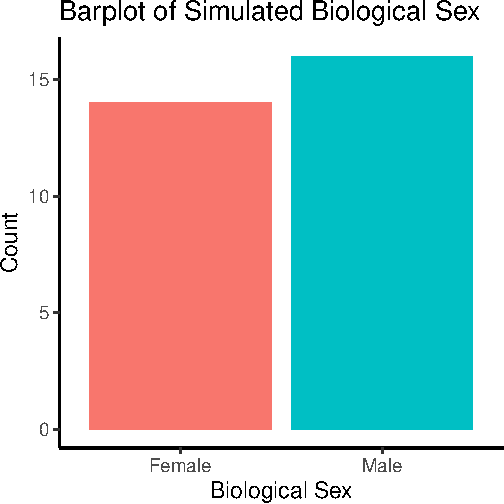
\includegraphics[width=0.5\linewidth]{02-descriptive-analysis_files/figure-latex/02-univar-sex-plot-1} 

}

\caption{Barplot of Biological Sex Responses}\label{fig:02-univar-sex-plot}
\end{figure}

\subsection{Gendered Aspect of Health Items}\label{gendered-aspect-of-health-items}

Looking at the density plots for \textbf{gender identity} and \textbf{gender role} (figure \ref{fig:02-univar-gi-plot}), we see that while both variables are bimodal, the \textbf{gender identity} responses is more strongly bimodal with one peak closer to the feminine side of the feminine-masculine continuum and one peak closer to masculine end of that continuum. Further, we can also see that in general, participants reported their \textbf{gender identity} and \textbf{roles} as being more feminine, again with the \textbf{gender identity} responses showing this trend more strongly than the \textbf{gender role} responses.

\begin{figure}

{\centering 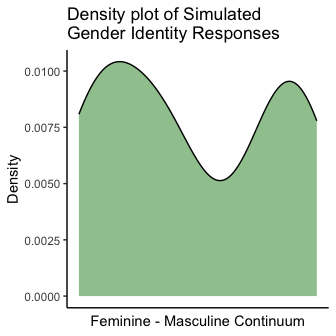
\includegraphics[width=0.5\linewidth]{02-descriptive-analysis_files/figure-latex/02-univar-gi-plot-1} 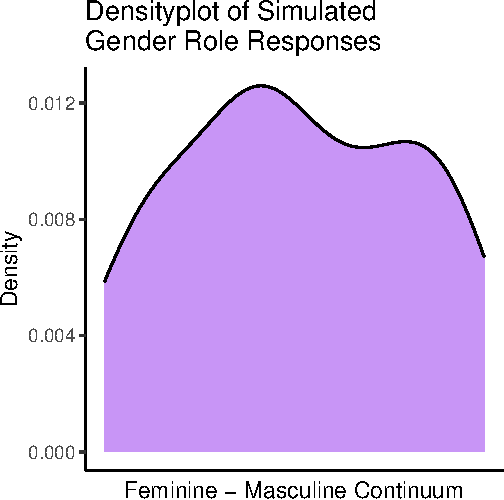
\includegraphics[width=0.5\linewidth]{02-descriptive-analysis_files/figure-latex/02-univar-gi-plot-2} 

}

\caption{Density plots of Gender Identity and Roles}\label{fig:02-univar-gi-plot}
\end{figure}

Presently, there is \emph{{no clear consensus on how to present descriptive statistics of bimodal variables in health research.}} Reporting the mean(sd) or median(IQR) of a variable does not clearly communicate that there is more than one peak in a bimodal variable's distribution.

When taken alongside the SGBA-5's assumption that the feminine-masculine continuum doesn't have a true 0 value, it is our suggestion that:

\begin{quote}
\emph{If researchers decide to report a descriptive statistic for a bimodally distributed variable, they should report a nominal description of the variable's distriubtion \textbf{skew}.}
\end{quote}

For example, if a gendered aspect of health item from the SGBA-5 demonstrates a bimodal distribution, the variable's \textbf{skew} can be described along the feminine-masculine continuum instead of reporting the numerical average alone.

To be able to describe the \textbf{skew} of one of the gender variables, the authors suggest calculating the variable's mean score along the feminine-masculine continuum and then reporting the skew using the suggested nominal classification guide seen in Table \ref{tab:02-tab}.

\emph{Please note that these suggested classification guidelines are arbitrary and may not be appropriate in all circumstances.}

\begin{table}

\caption{\label{tab:02-tab}Potential Interpretation of Sample Means for Gendered Aspect of Health Items.}
\centering
\begin{tabular}[t]{ll}
\toprule
Mean & Interpretation\\
\midrule
>70 & "Skews masculine"\\
55 to 70 & "More masculine than feminine"\\
45 to 55 & "Not strongly skewed"\\
30 to 45 & "More feminine than masculine"\\
<30 & "Skews feminine"\\
\bottomrule
\multicolumn{2}{l}{\textsuperscript{} This table assumes you have recorded the}\\
\multicolumn{2}{l}{gendered aspects of health items as 0}\\
\multicolumn{2}{l}{being the most feminine score and 100}\\
\multicolumn{2}{l}{being the most masculine score.}\\
\end{tabular}
\end{table}

For the simulated dataset represented in the density plots above, the mean score for the \textbf{gender identity} item was 50.2 and 46.8 for the \textbf{gender role} item. This means that when reporting descriptive statistics on the simulated sample we could report that: {\emph{``The simulated sample was not strongly skewed on a feminine to masculine continuum for either the gender identity or gender role measures from the SGBA-5''}}.

\section{Descriptive Table of SGBA-5 Responses}\label{descriptive-table-of-sgba-5-responses}

Taking all these together, an example of a sample characteristics table of the SGBA-5 items in the simulated dataset could be presented as has been displayed in Table \ref{tab:02-tab02}

\begin{table}

\caption{\label{tab:02-tab02}Simulated sample characteristics.}
\centering
\begin{tabular}[t]{ll}
\toprule
SGBA Item & Sample (n = 30)\\
\midrule
Biological Sex (n(\%)) & \\
<i>Female</i> & 14(47\%)\\
<i>Intersex</i> & NA\\
<i>Male</i> & 16(53\%)\\
Gendered Aspect of Health (skew) & \\
\addlinespace
<i>Gender Identity</i> & Not strongly skewed\\
<i>Gendered Roles</i> & Not strongly skewed\\
\bottomrule
\end{tabular}
\end{table}

\begin{quote}
See Appendix section \ref{sec:rcode-ch3} for the R code used in this chapter.
\end{quote}

\chapter{SGBA of a Continuous Variable}\label{continuous}

\begin{quote}
See Appendix section \ref{sec:rcode-ch4} for the R code used in this chapter.
\end{quote}

\begin{quote}
\emph{Note: for the biological sex and single gendered aspect of health item examples, an example outcome variable that demonstrates a relationship between that variable and the SGBA-5 item being assessed - the interaction example - and an example that does not demonstrate a relationship between itself and the SGBA-5 item - the no interaction example - is shown.}
\end{quote}

\section{Biological Sex}\label{biological-sex}

A good idea is to start by visualizing the continuous variable's distribution disaggregated by sex like the density plot in Figure \ref{fig:04-binary-pos-plot}. Then calculate disaggregated summary statistics for the continuous variable disaggregated by sex (Tables \ref{tab:03-tab-int} and \ref{tab:03-tab-no-int}), and conduct a statistical test of difference in means (Welch's t-test for this example).

\subsection{Density Plots by Biological Sex}\label{density-plots-by-biological-sex}

\begin{figure}

{\centering 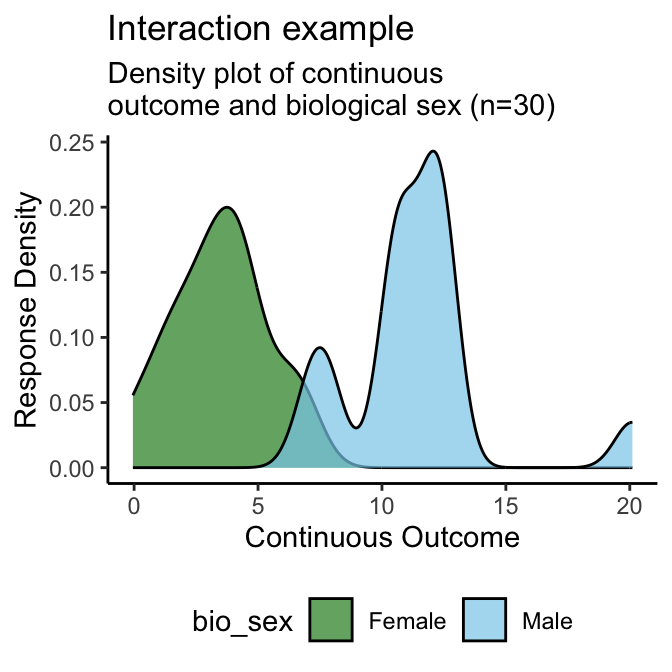
\includegraphics[width=0.5\linewidth]{03-continuous_files/figure-latex/04-binary-pos-plot-1} 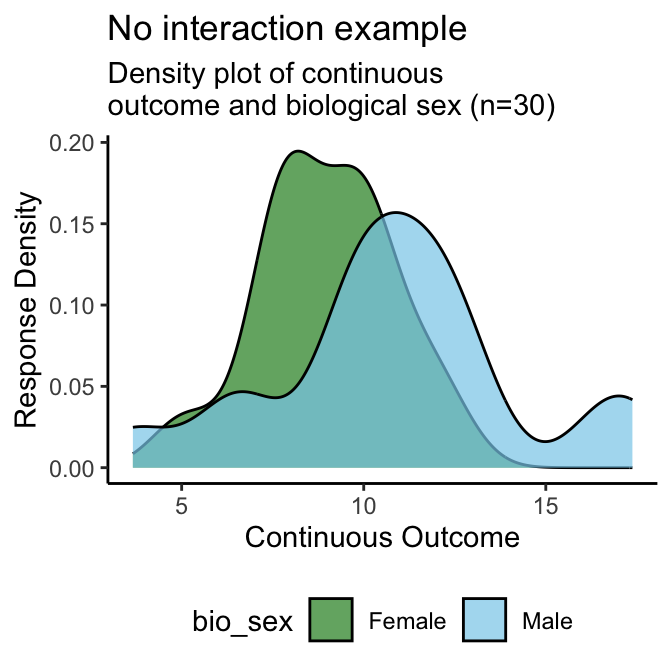
\includegraphics[width=0.5\linewidth]{03-continuous_files/figure-latex/04-binary-pos-plot-2} 

}

\caption{Density Plot of Continuous Variable by Biological Sex Examples}\label{fig:04-binary-pos-plot}
\end{figure}

\textbf{Interpretation:} From the above density plots (Figure \ref{fig:04-binary-pos-plot}) we can see a distinct overlap in the \textbf{no interaction example} which suggests that in that example's sample does not have a meaningful difference in the continuous outcome by sex. Conversely, the \textbf{interaction example} density plot has two distinct peaks which suggests that its sample's continuous outcome scores are associated with a participant's sex.

\subsection{Summary Statistics by Biological Sex}\label{summary-statistics-by-biological-sex}

\begin{table}

\caption{\label{tab:03-tab-int}Interation example summary statisitics: Continuous outcome and biological sex}
\centering
\begin{tabular}[t]{lrrrrr}
\toprule
biological sex & n & mean continuous & SD continuous & median continuous & IQR continuous\\
\midrule
Female & 14 & 3.5 & 1.94 & 4 & 2\\
Male & 16 & 11.3 & 2.95 & 11 & 2\\
\bottomrule
\end{tabular}
\end{table}

\begin{table}

\caption{\label{tab:03-tab-no-int}No interation example summary statisitics: Continuous outcome and biological sex}
\centering
\begin{tabular}[t]{lrrrrr}
\toprule
biological sex & n & mean continuous & SD continuous & median continuous & IQR continuous\\
\midrule
Female & 14 & 9.0 & 1.84 & 9 & 2\\
Male & 16 & 10.8 & 3.47 & 11 & 3\\
\bottomrule
\end{tabular}
\end{table}

\textbf{Interpretation:} As with the density plots, we see that the standard deviations of the continuous variable for both males and females overlap in the \textbf{no interaction example} (Table \ref{tab:03-tab-int}) - indicating a lack of significant difference by sex. The standard deviations of the continuous variable for both males and females do not overlap in the \textbf{interaction example} (Table \ref{tab:03-tab-no-int}) - indicating a potential association between that continuous outcome variable and sex.

\subsection{Statistical Testing of Biological Sex: t-test}\label{statistical-testing-of-biological-sex-t-test}

Next we will test the null hypothesis that biological sex does not have an impact on the continuous outcome variable being evaluated. Both the interaction example and no interaction example will be tested using a Welch's t-test at an alpha of .05.

\begin{quote}
\emph{Note: Using a Welch's t-test to test for statistically significant difference in these examples is a way, but by no means the only way in which this could be tested.}
\end{quote}

\begin{table}

\caption{\label{tab:04-tab-ttest}Statistical test of difference: Continuous outcome and biological sex.}
\centering
\begin{tabular}[t]{llrlrr}
\toprule
Example & Test & T-score & 95\% CI & df & p-value\\
\midrule
Interaction & Welch's t-test & -8.73 & (-9.72, -6.02) & 26.1 & 0.000\\
No interaction & Welch's t-test & -1.80 & (-3.85, 0.26) & 23.4 & 0.084\\
\bottomrule
\end{tabular}
\end{table}

\textbf{Interpretation:} Similarly to the descriptive table and density plots, we see that the \textbf{no interaction example} (Table \ref{tab:04-tab-ttest}) does not show a significant difference by sex (T=-1.80, 95\%CI=(-3.85,0.26), df=23.4, p-value\textgreater0.08). The \textbf{interaction example} (Table \ref{tab:04-tab-ttest}) shows a potential association between that continuous outcome variable and sex (T=-8.73, 95\%CI=(-9.82,-6.02), df=23.4, p-value\textless0.001), meriting further research into this potential interaction. This means that when reporting whether there was an association found between a continuous outcome and biological sex in the no interaction sample we can report that: {\emph{``The no interaction sample did not show evidence that biological sex was associated with the continuous outcome in this study''}}. Whereas the interaction sample, which did find a potential association, could report: {\emph{``The interaction sample found statistically significant evidence that biological sex was associated with the continuous outcome in this study''}}.

\subsection{Biological Sex: Interpretation Reporting Template}\label{biological-sex-interpretation-reporting-template}

Below are example templates for reporting whether an outcome variable is associated with biological sex as categorized by the SGBA-5. Replace the words in the square brackets to complete.

\begin{quote}
\textbf{If an association was found:}\\
In this study's sample we found that a person's self-reported biological sex at birth had a statistically significant association with {[}continuous variable name{]}. More detailed investigation of this relationship is required to directly interpret the potential effects this interaction.
\end{quote}

\begin{quote}
\textbf{If an association was not found:}\\
In this study's sample we found that a person's self-reported biological sex at birth did not show a statistically significant association with {[}continuous variable name{]}.
\end{quote}

\section{Gendered Aspects of Health: Assessing One Item}\label{gendered-aspects-of-health-assessing-one-item}

In this section we will analyze a single of the gendered aspects of health results from the SGBA-5 with a continuous variable of interest. Using the gender identity item as an example. First we will generate scatter (Figure \ref{fig:04-gi-scatter} ) and 2D-density plots (Figure \ref{fig:04-gi-2ddens}) of the continuous variable by the feminine-masculine continuum used in the SGBA-5. Then we shall calculate a Pearson correlation coefficient for that gendered aspect of health item and the continuous variable.

\subsection{Scatter \& 2-D Density Plots for One Item}\label{scatter-2-d-density-plots-for-one-item}

\begin{figure}

{\centering 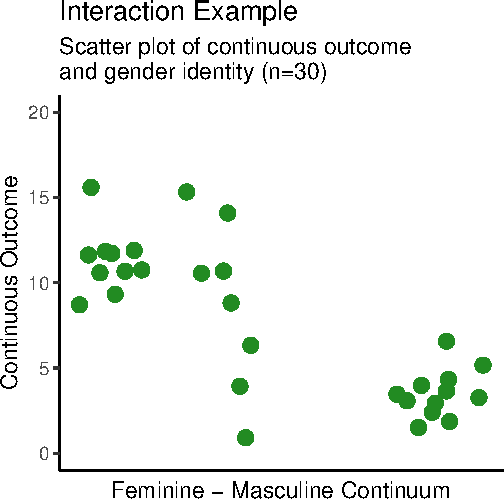
\includegraphics[width=0.5\linewidth]{03-continuous_files/figure-latex/04-gi-scatter-1} 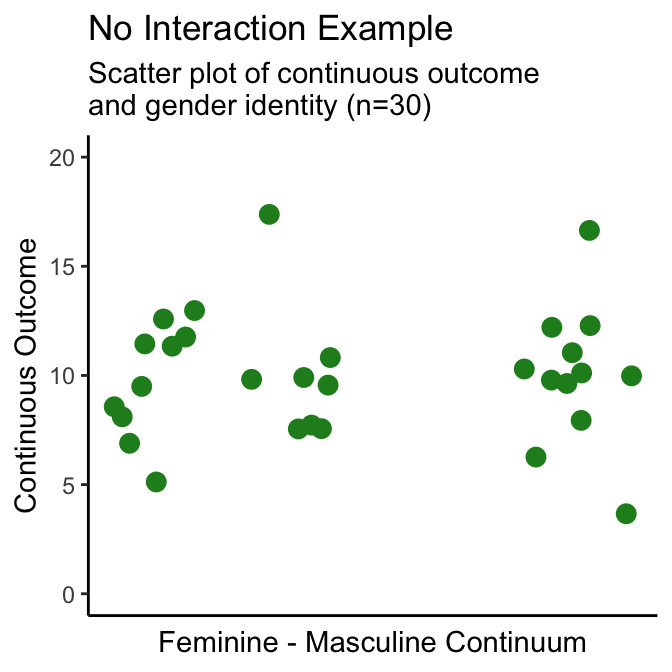
\includegraphics[width=0.5\linewidth]{03-continuous_files/figure-latex/04-gi-scatter-2} 

}

\caption{Scatter Plot of Continuous Variable by Gender Identity}\label{fig:04-gi-scatter}
\end{figure}

\begin{figure}

{\centering 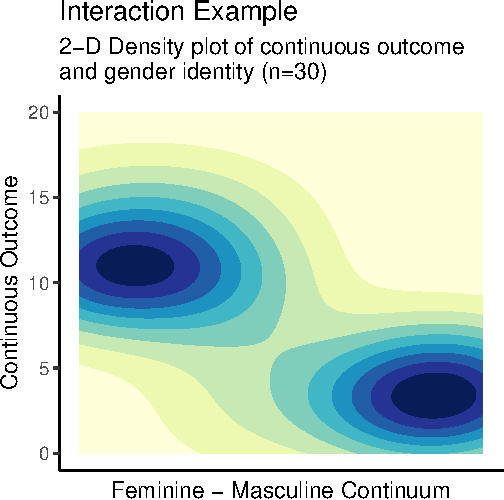
\includegraphics[width=0.5\linewidth]{03-continuous_files/figure-latex/04-gi-2ddens-1} 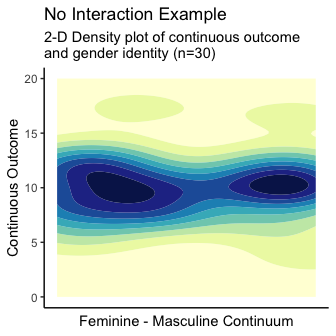
\includegraphics[width=0.5\linewidth]{03-continuous_files/figure-latex/04-gi-2ddens-2} 

}

\caption{2D Density Plots of Continuous Variable by Gender Identity}\label{fig:04-gi-2ddens}
\end{figure}

\textbf{Interpretation:} From the above scatter and 2-D density plots (Figures \ref{fig:04-gi-scatter} and \ref{fig:04-gi-2ddens}) we can see no clear pattern difference in the continuous outcome value across the feminine-masculine continuum in the \textbf{no interaction example} (i.e., the continuous outcome values of participants who are closer to the feminine end of the continuum are not noticeably different than participants who are not closer to the feminine end of the continuum). This suggests that the \textbf{no interaction example} does not show a meaningful difference in the continuous outcome by gender identity within this sample. Conversely, the \textbf{interaction example} scatter and 2-D density plots show two distinct clusters with the cluster closer to the feminine end of the continuum having higher continuous outcome values than the cluster closer to the masculine end of the continuum. This suggests that the \textbf{interaction example} sample's continuous outcome scores are associated with participants' self-reported place on the SGBA-5's feminine-masculine gender identity continuum.

\subsection{Summary Statistics for One Gendered Apsect of Health Item}\label{summary-statistics-for-one-gendered-apsect-of-health-item}

\begin{quote}
\emph{We do not recommend creating disaggregated summary statistics by any of the gendered aspects of health items from the SGBA-5. Analysis for effects associated with these variables can be conducted visually using plots (section \ref{scatter-2-d-density-plots-for-one-item}) or through statistical testing (section \ref{statistical-testing-for-one-item-pearsons-correlation-coefficient-r}).}
\end{quote}

\subsection{\texorpdfstring{Statistical Testing for One Item: Pearson's Correlation Coefficient (\emph{r})}{Statistical Testing for One Item: Pearson's Correlation Coefficient (r)}}\label{statistical-testing-for-one-item-pearsons-correlation-coefficient-r}

Next we will test the null hypothesis that a participant's self-reported gender identity on a feminine-masculine continuum does not have an impact on the continuous outcome variable being evaluated. Both the interaction example and no interaction example will be tested by calculating Pearson's Correlation Coefficient and describing that coefficient's strength and direction (\emph{{but not the exact coefficient value}}) as well as test for statistical significance of the correlation at an alpha of .05.

To be able to describe the strength of correlation between a continuous outcome and one of the gendered aspect of health variables, the authors suggest using a nominal classification of correlation strength. Using a nominal classification to interpret the strength of a correlation is inherently somewhat arbitrary, however, this trade-off can reduce potential misinterpretation that reporting a numerical coefficient value could cause. There maybe context- or discipline-specific guidelines for the interpretation of correlation strength which apply to your analysis. For the examples presented here, we will use the guidelines recommended in \href{https://doi.org/10.4324/9780203771587}{\emph{Statistical Power Analysis for the Behavioural Sciences} (2013) by Jacob Cohen}, which can be seen in Table \ref{tab:04-cohen}.

\emph{Please note that these suggested classification guidelines are arbitrary and may not be appropriate in all circumstances.}

\begin{table}

\caption{\label{tab:04-cohen}Nominal Interpretations of Correlation Strength.}
\centering
\begin{tabular}[t]{lll}
\toprule
Strength of Correlation & Positive Coefficient (r) & Negative Coefficient (r)\\
\midrule
None & 0.0 to 0.1 & 0.0 to -0.1\\
Weak & 0.1 to 0.3 & -0.1 to -0.3\\
Moderate & 0.3 to 0.5 & -0.3 to -0.5\\
Strong & 0.5 to 1.0 & -0.5 to -1.0\\
\bottomrule
\multicolumn{3}{l}{\textsuperscript{} Adapted from [\_Statistical Power Analysis for the Behavioural Sciences\_ (2013)}\\
\multicolumn{3}{l}{by Jacob Cohen](https://doi.org/10.4324/9780203771587)}\\
\end{tabular}
\end{table}

\begin{quote}
\emph{Note: Using Pearson's correlation coefficient to test for statistically significant difference in these examples is a way, but by no means the only way in which this could be tested.}
\end{quote}

\begin{table}

\caption{\label{tab:04-tab-r}Statistical test of difference: Continuous outcome and Gender Idenity Item from the SGBA-5.}
\centering
\begin{tabular}[t]{llrlrlrr}
\toprule
Example & Correlation Type & r & 95\% CI & df & Significance Test & T-score & p-value\\
\midrule
Interaction & Pearson's r & -0.80 & (-0.9, -0.61) & 28 & t-test & -6.96 & 0.000\\
No interaction & Pearson's r & 0.02 & (-0.34, 0.38) & 28 & t-test & 0.10 & 0.922\\
\bottomrule
\end{tabular}
\end{table}

\textbf{Interpretation:} The correlation coefficient we see for the \textbf{no interaction example} (Table \ref{tab:04-tab-r}) was 0.02. Using the classification criteria outlined in Table \ref{tab:04-cohen}, we see that the strength of correlation is ``None''. Thus, we can report that {\emph{``The no interaction sample did not show evidence of correlation between the gender identity item and the continuous outcome''}}. Similarly, we see that the \textbf{no interaction example}'s correlation does not meet the statistical significance threshold of 0.05 from the null hypothesis (T=0.10, df=28, p-value\textgreater0.9).

The \textbf{interaction example} shows a correlation coefficient of -0.80 (Table \ref{tab:04-tab-r}), which falls under the ``Strong'' category of correlation strength from Table \ref{tab:04-cohen}. Therefore, we could report that {\emph{``The interaction sample shows evidence of a strong correlation between the gender identity item and the continuous outcome''}}. Similarly, we see that the \textbf{interaction example}'s correlation exceeds the statistical significance threshold of 0.05 from the null hypothesis (T=-6.96, df=28, p-value\textless0.001).

\subsection{Gendered Aspects of Health: One Item Interpretation Reporting Template}\label{gendered-aspects-of-health-one-item-interpretation-reporting-template}

Below are example templates for reporting whether an outcome variable is associated with a gendered aspect of health as measured using the SGBA-5. Replace the words in the square brackets to complete.

\begin{quote}
\textbf{If an association was found:}\\
In this study's sample we found that a person's self-reported {[}gendered aspect of health item{]} had a statistically significant association with {[}continuous variable name{]}. More detailed investigation of this relationship is required to directly interpret the potential effects this interaction.
\end{quote}

\begin{quote}
\textbf{If an association was not found:}\\
In this study's sample we found that a person's self-reported {[}gendered aspect of health item{]} did not show a statistically significant association with {[}continuous variable name{]}.
\end{quote}

\section{Gendered Aspects of Health: Assessing Multiple Items}\label{gendered-aspects-of-health-assessing-multiple-items}

In this section we will show how an example of how you can analyze multiple gendered aspects of health results from the SGBA-5 with a continuous variable of interest. (Specifically, this example will demonstrate a SGBA using the gender identity and gender roles items from the SGBA-5. However, the process for assessing 3 of or all 4 items with a continuous variable can be extended from this example).

Like when assessing only one of the gendered aspect of health items, we will start by generating scatter (Figure \ref{fig:04-2gah-scatter} ) and 2D-density plots (Figure \ref{fig:04-2gah-2ddens}) of the continuous variable by the feminine-masculine continuum used in the SGBA-5. Then we shall calculate Pearson correlation coefficients between each gendered aspect of health item and the continuous variable.

\subsection{Scatter \& 2-D Density Plots for Two Items}\label{scatter-2-d-density-plots-for-two-items}

\begin{figure}

{\centering 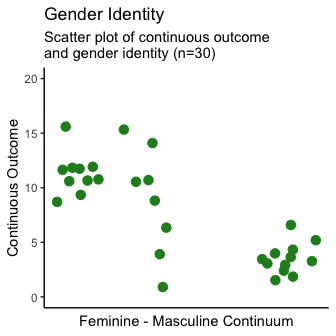
\includegraphics[width=0.5\linewidth]{03-continuous_files/figure-latex/04-2gah-scatter-1} 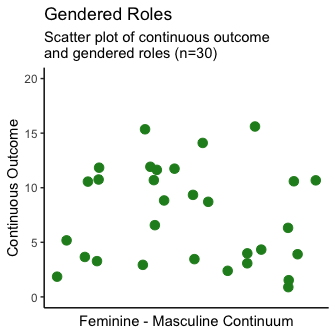
\includegraphics[width=0.5\linewidth]{03-continuous_files/figure-latex/04-2gah-scatter-2} 

}

\caption{Scatter Plot of Continuous Variable by Gender Identity and Gendered Roles}\label{fig:04-2gah-scatter}
\end{figure}

\begin{figure}

{\centering 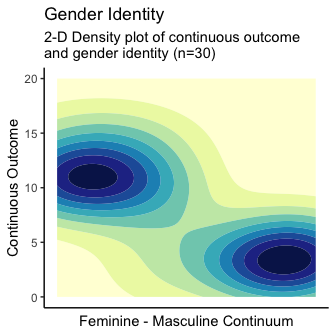
\includegraphics[width=0.5\linewidth]{03-continuous_files/figure-latex/04-2gah-2ddens-1} 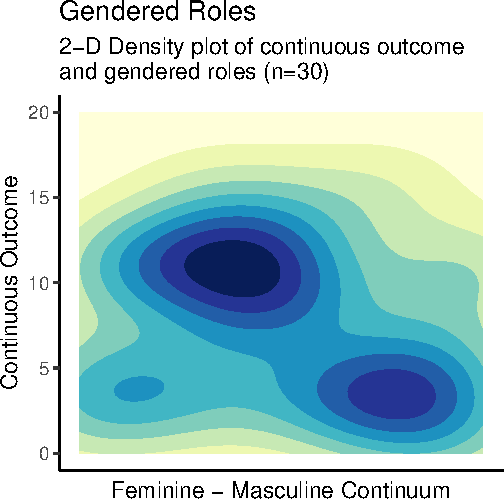
\includegraphics[width=0.5\linewidth]{03-continuous_files/figure-latex/04-2gah-2ddens-2} 

}

\caption{2D Density Plots of Continuous Variable by Gender Identityand Gendered Roles}\label{fig:04-2gah-2ddens}
\end{figure}

\textbf{Interpretation:} From the above scatter and 2-D density plots (Figures \ref{fig:04-2gah-scatter} and \ref{fig:04-2gah-2ddens}) we can see a relatively clear pattern difference in the continuous outcome value across the feminine-masculine continuum in the \textbf{gender identity} item. Whereas, the \textbf{gendered roles} item scatter and 2-D density plots show less distinct clustering with a cluster closer to the masculine end of the continuum having lower continuous outcome values and the continuous outcome values closer to the feminine end of the continuum showing both high and low values. This suggests that in this example the \textbf{gender identity} SGBA-5 item is associated with the continuous outcome variable in this example and the \textbf{gendered roles} item is not clear, but may suggest the potential of a more complicated relationship between the continuous outcome and \textbf{gendered roles}.

\subsection{Summary Statistics for Two Items}\label{summary-statistics-for-two-items}

\begin{quote}
\emph{As with assessing only one of the gendered aspects of health items from the SGBA-5, we do not recommend creating disaggregated summary statistics by any of the gendered aspects of health items from the SGBA-5. Analysis for effects associated with these variables can be conducted visually using plots (section \ref{scatter-2-d-density-plots-for-two-items}) or through statistical testing (section \ref{statistical-testing-for-two-items-pearsons-correlation-coefficient-r}).}
\end{quote}

\subsection{\texorpdfstring{Statistical Testing for Two Items: Pearson's Correlation Coefficient (\emph{r})}{Statistical Testing for Two Items: Pearson's Correlation Coefficient (r)}}\label{statistical-testing-for-two-items-pearsons-correlation-coefficient-r}

Next we will test the null hypothesis that a participant's self-reported gender identity or gendered roles on a feminine-masculine continuum do not impact the continuous outcome variable being evaluated.

\begin{quote}
\emph{Note: typically when conducting multiple comparisons we adjust the threshold for statistical significance to account for those multiple comparisons (e.g., using a Bonferroni Correction for calculating p-value thresholds). In the the example below we do not use a multiple comparison correction. This is because the calculated correlation values are assumed to be approximately indicative of an underlying association rather than interpretable as exact values. However, \textbf{if you intend to look at SGBA-5 items in comparison to multiple primary variables in your analysis we highly recommend adjusting your significance thresholds for multiple comparisons.}}
\end{quote}

Both the simulated gender identity and gendered roles SGBA-5 responses shown in the plots above will be tested for association with the continuous outcome variable by calculating Pearson's Correlation Coefficient and describing that coefficient's strength and direction (\emph{{but not the exact coefficient value}}) as well as test for statistical significance of the correlation at an alpha of .05.

As described previously in section \ref{statistical-testing-for-one-item-pearsons-correlation-coefficient-r}, the authors suggest using a nominal classification of correlation strength. For the examples presented here, we will use the guidelines recommended in \href{https://doi.org/10.4324/9780203771587}{\emph{Statistical Power Analysis for the Behavioural Sciences} (2013) by Jacob Cohen}, which is summarized in Table \ref{tab:04-cohen}.

\begin{quote}
\emph{Note: Using Pearson's correlation coefficient to test for statistically significant difference in these examples is a way, but by no means the only way in which this could be tested.}
\end{quote}

\begin{table}

\caption{\label{tab:04-2gah-tab-r}Statistical test of difference: Continuous outcome by Gender Idenity and Gendered Roles Items from the SGBA-5.}
\centering
\begin{tabular}[t]{llrlrlrr}
\toprule
Example & Correlation Type & r & 95\% CI & df & Significance Test & T-score & p-value\\
\midrule
Gender Identity & Pearson's r & -0.8 & (-0.9, -0.61) & 28 & t-test & -6.96 & 0.000\\
Gendered Roles & Pearson's r & -0.1 & (-0.45, 0.27) & 28 & t-test & -0.56 & 0.582\\
\bottomrule
\end{tabular}
\end{table}

\textbf{Interpretation:} The \textbf{gender identity} item shows a correlation coefficient of -0.80 (Table \ref{tab:04-2gah-tab-r}), which falls under the ``Strong'' category of correlation strength from Table \ref{tab:04-cohen}. Therefore, we could report that {\emph{``Our testing found evidence of a strong correlation between the gender identity item and the continuous outcome''}}. As we would expect given the strength of correlation, the \textbf{gender identity} item's correlation exceeds the statistical significance threshold of 0.05 from the null hypothesis (T=-6.96, df=28, p-value\textless0.001).

The correlation coefficient we see for the \textbf{gendered roles} item (Table \ref{tab:04-2gah-tab-r}) was -0.1. Using the classification criteria outlined in Table \ref{tab:04-cohen}, we see that the strength of correlation is on the border between ``None'' and ``Weak''. Airing on the side of caution, we can report that {\emph{``Our testing did not find clear evidence of correlation between the gendered roles item and the continuous outcome''}}. Similarly, we see that the \textbf{gendered roles} item's correlation does not meet the statistical significance threshold of 0.05 from the null hypothesis (T=-0.56, df=28, p-value\textgreater0.5).

\subsection{Gendered Aspects of Health: Multiple Item Interpretation Reporting Template}\label{gendered-aspects-of-health-multiple-item-interpretation-reporting-template}

Below are example templates for reporting whether an outcome variable is associated with gendered aspects of health as measured using the SGBA-5. Replace the words in the square brackets to complete.

\begin{quote}
\textbf{If associations were found for all of the gendered aspect of health items assessed:}\\
In this study's sample we found that a person's self-reported {[}gendered aspect of health items{]} demonstrated statistically significant associations with {[}continuous variable name{]}. More detailed investigation of these relationships is required to directly interpret the potential effects these interactions.
\end{quote}

\begin{quote}
\textbf{If associations were found for at least one of the gendered aspect of health items assessed:}\\
In this study's sample we found that a person's self-reported {[}gendered aspect of health items with association{]} demonstarted {[}a{]} statistically significant association{[}s{]} with {[}continuous variable name{]}, whereas a person's self-reported {[}gendered aspect of health items with no association{]} did not. More detailed investigation of these relationships is required to directly interpret the potential effects these interactions.
\end{quote}

\begin{quote}
\textbf{If no association was found:}\\
In this study's sample we found that a person's self-reported {[}gendered aspect of health items{]} did not show a statistically significant association with {[}continuous variable name{]}.
\end{quote}

\begin{quote}
See Appendix section \ref{sec:rcode-ch4} for the R code used in this chapter.
\end{quote}

\chapter{Appendix}\label{appendix}

\section{Simulated Data Creation}\label{sec:sim-data}

Below is the code used to create the simulated data that will be used to create the example SGBA seen throughout the rest of this example analysis.

\begin{Shaded}
\begin{Highlighting}[]
\CommentTok{\# load libraries {-}{-}{-}{-}{-}{-}{-}{-}{-}{-}{-}{-}{-}{-}{-}{-}{-}{-}{-}{-}{-}{-}{-}{-}{-}{-}{-}{-}{-}{-}{-}{-}{-}{-}{-}{-}{-}{-}{-}{-}{-}{-}{-}{-}{-}{-}{-}{-}{-}{-}{-}{-}{-}{-}{-}{-}{-}{-}}
\FunctionTok{library}\NormalTok{(tidyverse)}
\end{Highlighting}
\end{Shaded}

\begin{verbatim}
## -- Attaching core tidyverse packages -------------------------------------------- tidyverse 2.0.0 --
## v dplyr     1.1.4     v readr     2.1.5
## v forcats   1.0.0     v stringr   1.5.1
## v ggplot2   3.5.2     v tibble    3.3.0
## v lubridate 1.9.4     v tidyr     1.3.1
## v purrr     1.0.4     
## -- Conflicts -------------------------------------------------------------- tidyverse_conflicts() --
## x dplyr::filter() masks stats::filter()
## x dplyr::lag()    masks stats::lag()
## i Use the conflicted package (<http://conflicted.r-lib.org/>) to force all conflicts to become errors
\end{verbatim}

\begin{Shaded}
\begin{Highlighting}[]
\CommentTok{\# set seed for predictability}
\FunctionTok{set.seed}\NormalTok{(}\DecValTok{42}\NormalTok{, }\AttributeTok{kind =} \StringTok{"Mersenne{-}Twister"}\NormalTok{)}

\CommentTok{\# write simulation functions {-}{-}{-}{-}{-}{-}{-}{-}{-}{-}{-}{-}{-}{-}{-}{-}{-}{-}{-}{-}{-}{-}{-}{-}{-}{-}{-}{-}{-}{-}{-}{-}{-}{-}{-}{-}{-}{-}{-}{-}{-}{-}{-}{-}{-}{-}}

\CommentTok{\# function for simulating bimodal gender variables}
\NormalTok{binom\_bounded }\OtherTok{\textless{}{-}} \ControlFlowTok{function}\NormalTok{(}
\NormalTok{    n, prop, mean1, sd1, mean2, sd2, }\AttributeTok{lim\_low =} \SpecialCharTok{{-}}\ConstantTok{Inf}\NormalTok{, }\AttributeTok{lim\_up =} \ConstantTok{Inf}\NormalTok{, round}
\NormalTok{    )\{}
  \CommentTok{\# error checking}
  \ControlFlowTok{if}\NormalTok{(prop }\SpecialCharTok{\textgreater{}} \DecValTok{1} \SpecialCharTok{||}\NormalTok{ prop}\SpecialCharTok{\textless{}} \DecValTok{0}\NormalTok{)\{}\FunctionTok{stop}\NormalTok{(}\StringTok{"binomial proportion should be between 0 and 1"}\NormalTok{)\}}
  \ControlFlowTok{if}\NormalTok{(n }\SpecialCharTok{\textless{}} \DecValTok{1}\NormalTok{)\{}\FunctionTok{stop}\NormalTok{(}\StringTok{"n must be greater than or equal to 1"}\NormalTok{)\}}
  \ControlFlowTok{if}\NormalTok{(sd1 }\SpecialCharTok{\textless{}} \DecValTok{0} \SpecialCharTok{||}\NormalTok{ sd2 }\SpecialCharTok{\textless{}} \DecValTok{0}\NormalTok{)\{}\FunctionTok{stop}\NormalTok{(}\StringTok{"standard deviations must be non{-}negative"}\NormalTok{)\}}
  \CommentTok{\# create index}
\NormalTok{  index }\OtherTok{\textless{}{-}} \FunctionTok{rbinom}\NormalTok{(n, }\AttributeTok{size =} \DecValTok{1}\NormalTok{, }\AttributeTok{prob =}\NormalTok{ prop)}
  \CommentTok{\# simulate each peak using a bounded \textasciigrave{}rnorm()\textasciigrave{}}
\NormalTok{  binom\_sim1 }\OtherTok{\textless{}{-}}\NormalTok{ index }\SpecialCharTok{*} \FunctionTok{qnorm}\NormalTok{(}
    \FunctionTok{runif}\NormalTok{(}
\NormalTok{      n, }\FunctionTok{pnorm}\NormalTok{(lim\_low, mean1, sd1), }\FunctionTok{pnorm}\NormalTok{(lim\_up, mean1, sd1)}
\NormalTok{      ), }
\NormalTok{    mean1, sd1)}
\NormalTok{  binom\_sim0 }\OtherTok{\textless{}{-}}\NormalTok{ (}\DecValTok{1} \SpecialCharTok{{-}}\NormalTok{ index) }\SpecialCharTok{*} \FunctionTok{qnorm}\NormalTok{(}
    \FunctionTok{runif}\NormalTok{(}
\NormalTok{      n, }\FunctionTok{pnorm}\NormalTok{(lim\_low, mean2, sd2), }\FunctionTok{pnorm}\NormalTok{(lim\_up, mean2, sd2)}
\NormalTok{      ), }
\NormalTok{    mean2, sd2)}
\NormalTok{  binom\_sim }\OtherTok{\textless{}{-}}\NormalTok{ binom\_sim0 }\SpecialCharTok{+}\NormalTok{ binom\_sim1}
\NormalTok{  binom\_sim }\OtherTok{\textless{}{-}} \FunctionTok{round}\NormalTok{(binom\_sim, round)}
\NormalTok{  binom\_sim}
\NormalTok{\}}


\CommentTok{\# function for simulating Likert/ordinal outcome variable}
\NormalTok{ordinal\_sim }\OtherTok{\textless{}{-}} \ControlFlowTok{function}\NormalTok{(}
\NormalTok{    n, mean, sd, }\AttributeTok{lim\_low =} \SpecialCharTok{{-}}\ConstantTok{Inf}\NormalTok{, }\AttributeTok{lim\_up =} \ConstantTok{Inf}
\NormalTok{    )\{}
\NormalTok{  ord\_sim }\OtherTok{\textless{}{-}} \FunctionTok{qnorm}\NormalTok{(}
    \FunctionTok{runif}\NormalTok{(}
\NormalTok{      n, }\FunctionTok{pnorm}\NormalTok{(lim\_low, mean, sd), }\FunctionTok{pnorm}\NormalTok{(lim\_up, mean, sd)}
\NormalTok{      ),}
\NormalTok{    mean, sd)}
\NormalTok{  ord\_sim }\OtherTok{\textless{}{-}} \FunctionTok{round}\NormalTok{(ord\_sim, }\DecValTok{0}\NormalTok{)}
\NormalTok{  ord\_sim}
\NormalTok{\}}


\CommentTok{\# simulate SGBA{-}5 data with n of 30 {-}{-}{-}{-}{-}{-}{-}{-}{-}{-}{-}{-}{-}{-}{-}{-}{-}{-}{-}{-}{-}{-}{-}{-}{-}{-}{-}{-}{-}{-}{-}{-}{-}{-}{-}{-}{-}}

\CommentTok{\# biological sex: categorical (female, intersex, male)}
\NormalTok{bio\_sex }\OtherTok{\textless{}{-}} \FunctionTok{factor}\NormalTok{(}
  \FunctionTok{sample}\NormalTok{(}\FunctionTok{c}\NormalTok{(}\StringTok{\textquotesingle{}Female\textquotesingle{}}\NormalTok{, }\StringTok{\textquotesingle{}Male\textquotesingle{}}\NormalTok{), }\DecValTok{30}\NormalTok{, }\AttributeTok{replace=}\ConstantTok{TRUE}\NormalTok{, }\AttributeTok{prob=}\FunctionTok{c}\NormalTok{(}\FloatTok{0.6}\NormalTok{, }\FloatTok{0.4}\NormalTok{)),}
\NormalTok{  )}

\CommentTok{\# gender identity: ordered (0 [feminine] to 100 [masculine])}
\NormalTok{gen\_id }\OtherTok{\textless{}{-}} \FunctionTok{binom\_bounded}\NormalTok{(}
  \AttributeTok{n =} \DecValTok{30}\NormalTok{, }\AttributeTok{prop =} \FloatTok{0.6}\NormalTok{, }\AttributeTok{mean1 =} \DecValTok{20}\NormalTok{, }\AttributeTok{sd1 =} \DecValTok{20}\NormalTok{, }\AttributeTok{mean2 =} \DecValTok{85}\NormalTok{, }\AttributeTok{sd2 =} \DecValTok{15}\NormalTok{, }\AttributeTok{lim\_low =} \DecValTok{0}\NormalTok{,}
  \AttributeTok{lim\_up =} \DecValTok{100}\NormalTok{, }\AttributeTok{round =} \DecValTok{0}
\NormalTok{)}

\CommentTok{\# gender role: ordered (0 [feminine] to 100 [masculine])}
\NormalTok{gen\_role }\OtherTok{\textless{}{-}} \FunctionTok{binom\_bounded}\NormalTok{(}
  \AttributeTok{n =} \DecValTok{30}\NormalTok{, }\AttributeTok{prop =} \FloatTok{0.6}\NormalTok{, }\AttributeTok{mean1 =} \DecValTok{25}\NormalTok{, }\AttributeTok{sd1 =} \DecValTok{20}\NormalTok{, }\AttributeTok{mean2 =} \DecValTok{80}\NormalTok{, }\AttributeTok{sd2 =} \DecValTok{20}\NormalTok{, }\AttributeTok{lim\_low =} \DecValTok{0}\NormalTok{,}
  \AttributeTok{lim\_up =} \DecValTok{100}\NormalTok{, }\AttributeTok{round =} \DecValTok{0}
\NormalTok{)}


\CommentTok{\# simulate example positive outcome data with n of 30 {-}{-}{-}{-}{-}{-}{-}{-}{-}{-}{-}{-}{-}{-}{-}{-}{-}{-}{-}{-}{-}{-}{-}}

\DocumentationTok{\#\# simulated numerical outcome: {-}{-}{-}{-}{-}{-}{-}{-}{-}{-}{-}{-}{-}{-}{-}{-}{-}{-}{-}{-}{-}{-}{-}{-}{-}{-}{-}{-}{-}{-}{-}{-}{-}{-}{-}{-}{-}{-}{-}{-}{-}{-}{-}{-}}

\CommentTok{\# by sex: males (mean = 12, SD = 3), females (mean = 4, sd = 2)}
\NormalTok{outcome\_num\_pos\_m }\OtherTok{\textless{}{-}} \FunctionTok{rnorm}\NormalTok{(}\AttributeTok{n =} \DecValTok{16}\NormalTok{, }\AttributeTok{mean =} \DecValTok{12}\NormalTok{, }\AttributeTok{sd =} \DecValTok{3}\NormalTok{)}
\NormalTok{outcome\_num\_pos\_f }\OtherTok{\textless{}{-}} \FunctionTok{rnorm}\NormalTok{(}\AttributeTok{n =} \DecValTok{14}\NormalTok{, }\AttributeTok{mean =} \DecValTok{4}\NormalTok{, }\AttributeTok{sd =} \DecValTok{2}\NormalTok{)}
\NormalTok{outcome\_num\_pos\_sex }\OtherTok{\textless{}{-}} \FunctionTok{c}\NormalTok{(outcome\_num\_pos\_f, outcome\_num\_pos\_m)}

\CommentTok{\# by g\_id: high (mean = 12, SD = 3), low (mean = 4, sd = 2)}
\NormalTok{outcome\_num\_pos\_gid\_high }\OtherTok{\textless{}{-}} \FunctionTok{rnorm}\NormalTok{(}\AttributeTok{n =} \DecValTok{15}\NormalTok{, }\AttributeTok{mean =} \DecValTok{12}\NormalTok{, }\AttributeTok{sd =} \DecValTok{3}\NormalTok{)}
\NormalTok{outcome\_num\_pos\_gid\_low }\OtherTok{\textless{}{-}} \FunctionTok{rnorm}\NormalTok{(}\AttributeTok{n =} \DecValTok{15}\NormalTok{, }\AttributeTok{mean =} \DecValTok{4}\NormalTok{, }\AttributeTok{sd =} \DecValTok{2}\NormalTok{)}
\NormalTok{outcome\_num\_pos\_gid }\OtherTok{\textless{}{-}} \FunctionTok{c}\NormalTok{(outcome\_num\_pos\_gid\_high, outcome\_num\_pos\_gid\_low)}

\CommentTok{\# by g\_role: high (mean = 12, SD = 3), low (mean = 4, sd = 2)}
\NormalTok{outcome\_num\_pos\_grol\_high }\OtherTok{\textless{}{-}} \FunctionTok{rnorm}\NormalTok{(}\AttributeTok{n =} \DecValTok{12}\NormalTok{, }\AttributeTok{mean =} \DecValTok{12}\NormalTok{, }\AttributeTok{sd =} \DecValTok{3}\NormalTok{)}
\NormalTok{outcome\_num\_pos\_grol\_low }\OtherTok{\textless{}{-}} \FunctionTok{rnorm}\NormalTok{(}\AttributeTok{n =} \DecValTok{18}\NormalTok{, }\AttributeTok{mean =} \DecValTok{7}\NormalTok{, }\AttributeTok{sd =} \DecValTok{2}\NormalTok{)}
\NormalTok{outcome\_num\_pos\_grol }\OtherTok{\textless{}{-}} \FunctionTok{c}\NormalTok{(outcome\_num\_pos\_grol\_high, outcome\_num\_pos\_grol\_low)}


\DocumentationTok{\#\# simulated Likert outcome: {-}{-}{-}{-}{-}{-}{-}{-}{-}{-}{-}{-}{-}{-}{-}{-}{-}{-}{-}{-}{-}{-}{-}{-}{-}{-}{-}{-}{-}{-}{-}{-}{-}{-}{-}{-}{-}{-}{-}{-}{-}{-}{-}{-}{-}}

\CommentTok{\# by sex males (mean = 2, SD = 1), females (mean = 5, sd = 2)}
\NormalTok{outcome\_ord\_pos\_m }\OtherTok{\textless{}{-}} \FunctionTok{ordinal\_sim}\NormalTok{(}
  \AttributeTok{n =} \DecValTok{16}\NormalTok{, }\AttributeTok{mean =} \DecValTok{2}\NormalTok{, }\AttributeTok{sd =} \DecValTok{1}\NormalTok{, }\AttributeTok{lim\_low =} \DecValTok{1}\NormalTok{, }\AttributeTok{lim\_up =} \DecValTok{7}
\NormalTok{)}
\NormalTok{outcome\_ord\_pos\_f }\OtherTok{\textless{}{-}} \FunctionTok{ordinal\_sim}\NormalTok{(}
  \AttributeTok{n =} \DecValTok{14}\NormalTok{, }\AttributeTok{mean =} \DecValTok{5}\NormalTok{, }\AttributeTok{sd =} \DecValTok{1}\NormalTok{, }\AttributeTok{lim\_low =} \DecValTok{1}\NormalTok{, }\AttributeTok{lim\_up =} \DecValTok{7}
\NormalTok{)}
\NormalTok{outcome\_ord\_pos\_sex }\OtherTok{\textless{}{-}} \FunctionTok{c}\NormalTok{(outcome\_ord\_pos\_f, outcome\_ord\_pos\_m) }\SpecialCharTok{\%\textgreater{}\%}
  \FunctionTok{factor}\NormalTok{(., }\AttributeTok{levels =} \FunctionTok{c}\NormalTok{(}\DecValTok{1}\NormalTok{,}\DecValTok{2}\NormalTok{,}\DecValTok{3}\NormalTok{,}\DecValTok{4}\NormalTok{,}\DecValTok{5}\NormalTok{,}\DecValTok{6}\NormalTok{,}\DecValTok{7}\NormalTok{), }\AttributeTok{ordered =} \ConstantTok{TRUE}\NormalTok{)}


\CommentTok{\# by g\_id: high (mean = 5, SD = 2), low (mean = 1, sd = 2)}
\NormalTok{outcome\_ord\_pos\_high }\OtherTok{\textless{}{-}} \FunctionTok{ordinal\_sim}\NormalTok{(}
  \AttributeTok{n =} \DecValTok{15}\NormalTok{, }\AttributeTok{mean =} \DecValTok{5}\NormalTok{, }\AttributeTok{sd =} \DecValTok{2}\NormalTok{, }\AttributeTok{lim\_low =} \DecValTok{1}\NormalTok{, }\AttributeTok{lim\_up =} \DecValTok{7}
\NormalTok{)}
\NormalTok{outcome\_ord\_pos\_low }\OtherTok{\textless{}{-}} \FunctionTok{ordinal\_sim}\NormalTok{(}
  \AttributeTok{n =} \DecValTok{15}\NormalTok{, }\AttributeTok{mean =} \DecValTok{1}\NormalTok{, }\AttributeTok{sd =} \DecValTok{2}\NormalTok{, }\AttributeTok{lim\_low =} \DecValTok{1}\NormalTok{, }\AttributeTok{lim\_up =} \DecValTok{7}
\NormalTok{)}
\NormalTok{outcome\_ord\_pos\_gid }\OtherTok{\textless{}{-}} \FunctionTok{c}\NormalTok{(outcome\_ord\_pos\_high, outcome\_ord\_pos\_low) }\SpecialCharTok{\%\textgreater{}\%}
  \FunctionTok{factor}\NormalTok{(., }\AttributeTok{levels =} \FunctionTok{c}\NormalTok{(}\DecValTok{1}\NormalTok{,}\DecValTok{2}\NormalTok{,}\DecValTok{3}\NormalTok{,}\DecValTok{4}\NormalTok{,}\DecValTok{5}\NormalTok{,}\DecValTok{6}\NormalTok{,}\DecValTok{7}\NormalTok{), }\AttributeTok{ordered =} \ConstantTok{TRUE}\NormalTok{)}


\CommentTok{\# by g\_role: high (mean = 5, SD = 2), low (mean = 1, sd = 2)}
\NormalTok{outcome\_ord\_pos\_high }\OtherTok{\textless{}{-}} \FunctionTok{ordinal\_sim}\NormalTok{(}
  \AttributeTok{n =} \DecValTok{12}\NormalTok{, }\AttributeTok{mean =} \DecValTok{5}\NormalTok{, }\AttributeTok{sd =} \DecValTok{2}\NormalTok{, }\AttributeTok{lim\_low =} \DecValTok{1}\NormalTok{, }\AttributeTok{lim\_up =} \DecValTok{7}
\NormalTok{)}
\NormalTok{outcome\_ord\_pos\_low }\OtherTok{\textless{}{-}} \FunctionTok{ordinal\_sim}\NormalTok{(}
  \AttributeTok{n =} \DecValTok{18}\NormalTok{, }\AttributeTok{mean =} \DecValTok{1}\NormalTok{, }\AttributeTok{sd =} \DecValTok{2}\NormalTok{, }\AttributeTok{lim\_low =} \DecValTok{1}\NormalTok{, }\AttributeTok{lim\_up =} \DecValTok{7}
\NormalTok{)}
\NormalTok{outcome\_ord\_pos\_grol }\OtherTok{\textless{}{-}} \FunctionTok{c}\NormalTok{(outcome\_ord\_pos\_high, outcome\_ord\_pos\_low) }\SpecialCharTok{\%\textgreater{}\%}
  \FunctionTok{factor}\NormalTok{(., }\AttributeTok{levels =} \FunctionTok{c}\NormalTok{(}\DecValTok{1}\NormalTok{,}\DecValTok{2}\NormalTok{,}\DecValTok{3}\NormalTok{,}\DecValTok{4}\NormalTok{,}\DecValTok{5}\NormalTok{,}\DecValTok{6}\NormalTok{,}\DecValTok{7}\NormalTok{), }\AttributeTok{ordered =} \ConstantTok{TRUE}\NormalTok{)}


\DocumentationTok{\#\# simulated binary outcome: {-}{-}{-}{-}{-}{-}{-}{-}{-}{-}{-}{-}{-}{-}{-}{-}{-}{-}{-}{-}{-}{-}{-}{-}{-}{-}{-}{-}{-}{-}{-}{-}{-}{-}{-}{-}{-}{-}{-}{-}{-}{-}{-}{-}{-}{-}{-}}

\CommentTok{\# by sex males (yes = .2, no = .8), females (yes = .8, no = .2)}
\NormalTok{outcome\_bin\_pos\_m }\OtherTok{\textless{}{-}} \FunctionTok{sample}\NormalTok{(}
  \FunctionTok{c}\NormalTok{(}\StringTok{\textquotesingle{}yes\textquotesingle{}}\NormalTok{,}\StringTok{\textquotesingle{}no\textquotesingle{}}\NormalTok{), }\DecValTok{16}\NormalTok{, }\AttributeTok{replace =} \ConstantTok{TRUE}\NormalTok{, }\AttributeTok{prob =} \FunctionTok{c}\NormalTok{(.}\DecValTok{2}\NormalTok{, .}\DecValTok{8}\NormalTok{)}
\NormalTok{)}
\NormalTok{outcome\_bin\_pos\_f }\OtherTok{\textless{}{-}} \FunctionTok{sample}\NormalTok{(}
  \FunctionTok{c}\NormalTok{(}\StringTok{\textquotesingle{}yes\textquotesingle{}}\NormalTok{,}\StringTok{\textquotesingle{}no\textquotesingle{}}\NormalTok{), }\DecValTok{14}\NormalTok{, }\AttributeTok{replace =} \ConstantTok{TRUE}\NormalTok{, }\AttributeTok{prob =} \FunctionTok{c}\NormalTok{(.}\DecValTok{8}\NormalTok{, .}\DecValTok{2}\NormalTok{)}
\NormalTok{)}
\NormalTok{outcome\_bin\_pos\_sex }\OtherTok{\textless{}{-}} \FunctionTok{append}\NormalTok{(outcome\_bin\_pos\_f, outcome\_bin\_pos\_m) }\SpecialCharTok{\%\textgreater{}\%}
  \FunctionTok{factor}\NormalTok{()}


\CommentTok{\# by g\_id: high (yes = .4, no = .6), low (yes = .8, no = .2)}
\NormalTok{outcome\_bin\_pos\_high }\OtherTok{\textless{}{-}} \FunctionTok{sample}\NormalTok{(}
  \FunctionTok{c}\NormalTok{(}\StringTok{\textquotesingle{}yes\textquotesingle{}}\NormalTok{,}\StringTok{\textquotesingle{}no\textquotesingle{}}\NormalTok{), }\DecValTok{15}\NormalTok{, }\AttributeTok{replace =} \ConstantTok{TRUE}\NormalTok{, }\AttributeTok{prob =} \FunctionTok{c}\NormalTok{(.}\DecValTok{4}\NormalTok{, .}\DecValTok{6}\NormalTok{)}
\NormalTok{)}
\NormalTok{outcome\_bin\_pos\_low }\OtherTok{\textless{}{-}} \FunctionTok{sample}\NormalTok{(}
  \FunctionTok{c}\NormalTok{(}\StringTok{\textquotesingle{}yes\textquotesingle{}}\NormalTok{,}\StringTok{\textquotesingle{}no\textquotesingle{}}\NormalTok{), }\DecValTok{15}\NormalTok{, }\AttributeTok{replace =} \ConstantTok{TRUE}\NormalTok{, }\AttributeTok{prob =} \FunctionTok{c}\NormalTok{(.}\DecValTok{8}\NormalTok{, .}\DecValTok{2}\NormalTok{)}
\NormalTok{)}
\NormalTok{outcome\_bin\_pos\_gid }\OtherTok{\textless{}{-}} \FunctionTok{append}\NormalTok{(outcome\_bin\_pos\_high, outcome\_bin\_pos\_low) }\SpecialCharTok{\%\textgreater{}\%}
  \FunctionTok{factor}\NormalTok{()}


\CommentTok{\# by g\_rol: high (yes = .3, no = .5), low (yes = .8, no = .2)}
\NormalTok{outcome\_bin\_pos\_high }\OtherTok{\textless{}{-}} \FunctionTok{sample}\NormalTok{(}
  \FunctionTok{c}\NormalTok{(}\StringTok{\textquotesingle{}yes\textquotesingle{}}\NormalTok{,}\StringTok{\textquotesingle{}no\textquotesingle{}}\NormalTok{), }\DecValTok{12}\NormalTok{, }\AttributeTok{replace =} \ConstantTok{TRUE}\NormalTok{, }\AttributeTok{prob =} \FunctionTok{c}\NormalTok{(.}\DecValTok{3}\NormalTok{, .}\DecValTok{7}\NormalTok{)}
\NormalTok{)}
\NormalTok{outcome\_bin\_pos\_low }\OtherTok{\textless{}{-}} \FunctionTok{sample}\NormalTok{(}
  \FunctionTok{c}\NormalTok{(}\StringTok{\textquotesingle{}yes\textquotesingle{}}\NormalTok{,}\StringTok{\textquotesingle{}no\textquotesingle{}}\NormalTok{), }\DecValTok{18}\NormalTok{, }\AttributeTok{replace =} \ConstantTok{TRUE}\NormalTok{, }\AttributeTok{prob =} \FunctionTok{c}\NormalTok{(.}\DecValTok{8}\NormalTok{, .}\DecValTok{2}\NormalTok{)}
\NormalTok{)}
\NormalTok{outcome\_bin\_pos\_grol }\OtherTok{\textless{}{-}} \FunctionTok{append}\NormalTok{(outcome\_bin\_pos\_high, outcome\_bin\_pos\_low) }\SpecialCharTok{\%\textgreater{}\%}
  \FunctionTok{factor}\NormalTok{()}


\CommentTok{\# simulate example negative outcome data with n of 30 {-}{-}{-}{-}{-}{-}{-}{-}{-}{-}{-}{-}{-}{-}{-}{-}{-}{-}{-}{-}{-}{-}{-}}

\CommentTok{\# simulated numerical outcome: continuous (mean = 10, SD = 3)}
\NormalTok{outcome\_num\_neg }\OtherTok{\textless{}{-}} \FunctionTok{rnorm}\NormalTok{(}\AttributeTok{n =} \DecValTok{30}\NormalTok{, }\AttributeTok{mean =} \DecValTok{10}\NormalTok{, }\AttributeTok{sd =} \DecValTok{3}\NormalTok{)}

\CommentTok{\# simulated Likert outcome: 7{-}point Likert scale (mean = 4, SD = 2)}
\NormalTok{outcome\_ord\_neg }\OtherTok{\textless{}{-}} \FunctionTok{ordinal\_sim}\NormalTok{(}
  \AttributeTok{n =} \DecValTok{30}\NormalTok{, }\AttributeTok{mean =} \DecValTok{4}\NormalTok{, }\AttributeTok{sd =} \DecValTok{2}\NormalTok{, }\AttributeTok{lim\_low =} \DecValTok{1}\NormalTok{, }\AttributeTok{lim\_up =} \DecValTok{7}
\NormalTok{)}

\CommentTok{\# simulated binary outcome: categorical (yes, no)}
\NormalTok{outcome\_bin\_neg }\OtherTok{\textless{}{-}} \FunctionTok{factor}\NormalTok{(}
  \FunctionTok{sample}\NormalTok{(}\FunctionTok{c}\NormalTok{(}\StringTok{\textquotesingle{}yes\textquotesingle{}}\NormalTok{,}\StringTok{\textquotesingle{}no\textquotesingle{}}\NormalTok{), }\DecValTok{30}\NormalTok{, }\AttributeTok{replace =} \ConstantTok{TRUE}\NormalTok{, }\AttributeTok{prob =} \FunctionTok{c}\NormalTok{(}\FloatTok{0.67}\NormalTok{, }\FloatTok{0.33}\NormalTok{))}
\NormalTok{)}


\CommentTok{\# create example data frame {-}{-}{-}{-}{-}{-}{-}{-}{-}{-}{-}{-}{-}{-}{-}{-}{-}{-}{-}{-}{-}{-}{-}{-}{-}{-}{-}{-}{-}{-}{-}{-}{-}{-}{-}{-}{-}{-}{-}{-}{-}{-}{-}{-}{-}{-}{-}}

\CommentTok{\# combine into dataframe}
\NormalTok{sim\_data }\OtherTok{\textless{}{-}} \FunctionTok{tibble}\NormalTok{(}
\NormalTok{  bio\_sex, gen\_id, gen\_role, }\CommentTok{\#outcome\_bin\_pos, }
\NormalTok{  outcome\_num\_neg, outcome\_ord\_neg, outcome\_bin\_neg}
\NormalTok{  ) }\SpecialCharTok{\%\textgreater{}\%} \FunctionTok{arrange}\NormalTok{(., bio\_sex) }\SpecialCharTok{\%\textgreater{}\%} 
  \FunctionTok{cbind}\NormalTok{(., outcome\_num\_pos\_sex) }\SpecialCharTok{\%\textgreater{}\%}
  \FunctionTok{cbind}\NormalTok{(., outcome\_ord\_pos\_sex) }\SpecialCharTok{\%\textgreater{}\%}
  \FunctionTok{cbind}\NormalTok{(., outcome\_bin\_pos\_sex) }\SpecialCharTok{\%\textgreater{}\%}
  \FunctionTok{arrange}\NormalTok{(., gen\_id) }\SpecialCharTok{\%\textgreater{}\%} 
  \FunctionTok{cbind}\NormalTok{(., outcome\_num\_pos\_gid) }\SpecialCharTok{\%\textgreater{}\%} 
  \FunctionTok{cbind}\NormalTok{(., outcome\_ord\_pos\_gid) }\SpecialCharTok{\%\textgreater{}\%}
  \FunctionTok{cbind}\NormalTok{(., outcome\_bin\_pos\_gid) }\SpecialCharTok{\%\textgreater{}\%}
  \FunctionTok{arrange}\NormalTok{(., gen\_role) }\SpecialCharTok{\%\textgreater{}\%} 
  \FunctionTok{cbind}\NormalTok{(., outcome\_num\_pos\_grol) }\SpecialCharTok{\%\textgreater{}\%} 
  \FunctionTok{cbind}\NormalTok{(., outcome\_ord\_pos\_grol) }\SpecialCharTok{\%\textgreater{}\%}
  \FunctionTok{cbind}\NormalTok{(., outcome\_bin\_pos\_grol)}


\CommentTok{\# save simulated df}
\FunctionTok{write\_csv}\NormalTok{(sim\_data, }\AttributeTok{file =} \StringTok{"sim{-}data.csv"}\NormalTok{)}
\end{Highlighting}
\end{Shaded}

\subsection{Session Info for Data Creation}\label{session-info-for-data-creation}

\begin{Shaded}
\begin{Highlighting}[]
\NormalTok{sessioninfo}\SpecialCharTok{::}\FunctionTok{session\_info}\NormalTok{(}\AttributeTok{pkgs =} \StringTok{"loaded"}\NormalTok{)}
\end{Highlighting}
\end{Shaded}

\begin{verbatim}
## - Session info -----------------------------------------------------------------------------------
##  setting  value
##  version  R version 4.5.0 (2025-04-11)
##  os       macOS Sequoia 15.5
##  system   aarch64, darwin20
##  ui       X11
##  language (EN)
##  collate  en_US.UTF-8
##  ctype    en_US.UTF-8
##  tz       America/Toronto
##  date     2025-07-26
##  pandoc   3.4 @ /Applications/RStudio.app/Contents/Resources/app/quarto/bin/tools/aarch64/ (via rmarkdown)
##  quarto   1.6.42 @ /Applications/RStudio.app/Contents/Resources/app/quarto/bin/quarto
## 
## - Packages ---------------------------------------------------------------------------------------
##  package      * version date (UTC) lib source
##  bit            4.6.0   2025-03-06 [1] CRAN (R 4.5.0)
##  bit64          4.6.0-1 2025-01-16 [1] CRAN (R 4.5.0)
##  bookdown       0.43    2025-04-15 [1] CRAN (R 4.5.0)
##  cli            3.6.5   2025-04-23 [1] CRAN (R 4.5.0)
##  crayon         1.5.3   2024-06-20 [1] CRAN (R 4.5.0)
##  digest         0.6.37  2024-08-19 [1] CRAN (R 4.5.0)
##  dplyr        * 1.1.4   2023-11-17 [1] CRAN (R 4.5.0)
##  evaluate       1.0.4   2025-06-18 [1] CRAN (R 4.5.0)
##  farver         2.1.2   2024-05-13 [1] CRAN (R 4.5.0)
##  fastmap        1.2.0   2024-05-15 [1] CRAN (R 4.5.0)
##  forcats      * 1.0.0   2023-01-29 [1] CRAN (R 4.5.0)
##  generics       0.1.4   2025-05-09 [1] CRAN (R 4.5.0)
##  ggplot2      * 3.5.2   2025-04-09 [1] CRAN (R 4.5.0)
##  glue           1.8.0   2024-09-30 [1] CRAN (R 4.5.0)
##  gtable         0.3.6   2024-10-25 [1] CRAN (R 4.5.0)
##  hms            1.1.3   2023-03-21 [1] CRAN (R 4.5.0)
##  htmltools      0.5.8.1 2024-04-04 [1] CRAN (R 4.5.0)
##  knitr          1.50    2025-03-16 [1] CRAN (R 4.5.0)
##  lifecycle      1.0.4   2023-11-07 [1] CRAN (R 4.5.0)
##  lubridate    * 1.9.4   2024-12-08 [1] CRAN (R 4.5.0)
##  magrittr       2.0.3   2022-03-30 [1] CRAN (R 4.5.0)
##  pillar         1.11.0  2025-07-04 [1] CRAN (R 4.5.0)
##  pkgconfig      2.0.3   2019-09-22 [1] CRAN (R 4.5.0)
##  purrr        * 1.0.4   2025-02-05 [1] CRAN (R 4.5.0)
##  R6             2.6.1   2025-02-15 [1] CRAN (R 4.5.0)
##  RColorBrewer   1.1-3   2022-04-03 [1] CRAN (R 4.5.0)
##  readr        * 2.1.5   2024-01-10 [1] CRAN (R 4.5.0)
##  rlang          1.1.6   2025-04-11 [1] CRAN (R 4.5.0)
##  rmarkdown      2.29    2024-11-04 [1] CRAN (R 4.5.0)
##  rstudioapi     0.17.1  2024-10-22 [1] CRAN (R 4.5.0)
##  scales         1.4.0   2025-04-24 [1] CRAN (R 4.5.0)
##  sessioninfo    1.2.3   2025-02-05 [1] CRAN (R 4.5.0)
##  stringi        1.8.7   2025-03-27 [1] CRAN (R 4.5.0)
##  stringr      * 1.5.1   2023-11-14 [1] CRAN (R 4.5.0)
##  tibble       * 3.3.0   2025-06-08 [1] CRAN (R 4.5.0)
##  tidyr        * 1.3.1   2024-01-24 [1] CRAN (R 4.5.0)
##  tidyselect     1.2.1   2024-03-11 [1] CRAN (R 4.5.0)
##  tidyverse    * 2.0.0   2023-02-22 [1] CRAN (R 4.5.0)
##  timechange     0.3.0   2024-01-18 [1] CRAN (R 4.5.0)
##  tzdb           0.5.0   2025-03-15 [1] CRAN (R 4.5.0)
##  vctrs          0.6.5   2023-12-01 [1] CRAN (R 4.5.0)
##  vroom          1.6.5   2023-12-05 [1] CRAN (R 4.5.0)
##  withr          3.0.2   2024-10-28 [1] CRAN (R 4.5.0)
##  xfun           0.52    2025-04-02 [1] CRAN (R 4.5.0)
##  yaml           2.3.10  2024-07-26 [1] CRAN (R 4.5.0)
## 
##  [1] /Library/Frameworks/R.framework/Versions/4.5-arm64/Resources/library
##  * -- Packages attached to the search path.
## 
## --------------------------------------------------------------------------------------------------
\end{verbatim}

\section{Ch. 3 Descriptive Analysis}\label{sec:rcode-ch3}

\subsection{Ch. 3 Set Up}\label{ch.-3-set-up}

\begin{Shaded}
\begin{Highlighting}[]
\CommentTok{\# load libraries and simulated data {-}{-}{-}{-}{-}{-}{-}{-}{-}{-}{-}{-}{-}{-}{-}{-}{-}{-}{-}{-}{-}{-}{-}{-}{-}{-}{-}{-}{-}{-}{-}{-}{-}{-}{-}{-}{-}{-}{-}}
\FunctionTok{library}\NormalTok{(tidyverse)}
\FunctionTok{library}\NormalTok{(ggpubr)}

\CommentTok{\# set seed for reproducibility}
\FunctionTok{set.seed}\NormalTok{(}\DecValTok{42}\NormalTok{)}

\CommentTok{\# load data set (from RDS if using previous script to simulate the data)}
\NormalTok{sim\_data }\OtherTok{\textless{}{-}} \FunctionTok{read\_csv}\NormalTok{(}\AttributeTok{file =} \StringTok{"sim{-}data.csv"}\NormalTok{)}

\CommentTok{\# default density plots and scale function {-}{-}{-}{-}{-}{-}{-}{-}{-}{-}{-}{-}{-}{-}{-}{-}{-}{-}{-}{-}{-}{-}{-}{-}{-}{-}{-}{-}{-}{-}{-}{-}{-}{-}}
\NormalTok{plot\_dens\_2D }\OtherTok{\textless{}{-}} \ControlFlowTok{function}\NormalTok{(data, x, y)\{}
\NormalTok{  plot }\OtherTok{\textless{}{-}} \FunctionTok{ggplot}\NormalTok{(}\AttributeTok{data =}\NormalTok{ data, }\FunctionTok{aes}\NormalTok{(}\AttributeTok{x =}\NormalTok{ x, }\AttributeTok{y =}\NormalTok{ y)) }\SpecialCharTok{+} 
    \FunctionTok{geom\_density\_2d\_filled}\NormalTok{(}\FunctionTok{aes}\NormalTok{(}\AttributeTok{fill =} \FunctionTok{after\_stat}\NormalTok{(level)),}
                           \AttributeTok{bins =} \DecValTok{9}\NormalTok{, }\AttributeTok{contour\_var =} \StringTok{\textquotesingle{}ndensity\textquotesingle{}}\NormalTok{) }\SpecialCharTok{+}
    \FunctionTok{scale\_fill\_brewer}\NormalTok{(}\AttributeTok{palette =} \DecValTok{16}\NormalTok{, }\AttributeTok{direction =} \DecValTok{1}\NormalTok{, }
                      \AttributeTok{labels =} \FunctionTok{c}\NormalTok{(}\StringTok{\textquotesingle{}Low\textquotesingle{}}\NormalTok{, }\StringTok{\textquotesingle{}\textquotesingle{}}\NormalTok{, }\StringTok{\textquotesingle{}\textquotesingle{}}\NormalTok{, }\StringTok{\textquotesingle{}\textquotesingle{}}\NormalTok{,}\StringTok{\textquotesingle{}\textquotesingle{}}\NormalTok{,}\StringTok{\textquotesingle{}\textquotesingle{}}\NormalTok{,}\StringTok{\textquotesingle{}\textquotesingle{}}\NormalTok{,}\StringTok{\textquotesingle{}\textquotesingle{}}\NormalTok{, }\StringTok{\textquotesingle{}High\textquotesingle{}}\NormalTok{)) }\SpecialCharTok{+}
    \FunctionTok{guides}\NormalTok{(}\AttributeTok{fill =} \FunctionTok{guide\_legend}\NormalTok{(}\AttributeTok{title =} \StringTok{\textquotesingle{}Density of Occurences\textquotesingle{}}\NormalTok{, }
                               \AttributeTok{direction =} \StringTok{\textquotesingle{}horizontal\textquotesingle{}}\NormalTok{, }\AttributeTok{nrow =} \DecValTok{1}\NormalTok{, }
                               \AttributeTok{label.position =} \StringTok{\textquotesingle{}bottom\textquotesingle{}}\NormalTok{))}
\NormalTok{  plot}
\NormalTok{\}}
\end{Highlighting}
\end{Shaded}

\subsection{Figure 3.1}\label{figure-3.1}

\begin{Shaded}
\begin{Highlighting}[]
\CommentTok{\# biological sex bar plot}
\FunctionTok{ggplot}\NormalTok{(sim\_data, }\FunctionTok{aes}\NormalTok{(}\AttributeTok{x =}\NormalTok{ bio\_sex)) }\SpecialCharTok{+}
  \FunctionTok{geom\_bar}\NormalTok{(}\FunctionTok{aes}\NormalTok{(}\AttributeTok{fill =}\NormalTok{ bio\_sex), }\AttributeTok{show.legend =}\NormalTok{ F) }\SpecialCharTok{+} 
  \FunctionTok{labs}\NormalTok{(}\AttributeTok{title =} \StringTok{\textquotesingle{}Barplot of Simulated Biological Sex\textquotesingle{}}\NormalTok{) }\SpecialCharTok{+}
  \FunctionTok{ylab}\NormalTok{(}\StringTok{\textquotesingle{}Count\textquotesingle{}}\NormalTok{) }\SpecialCharTok{+} \FunctionTok{xlab}\NormalTok{(}\StringTok{\textquotesingle{}Biological Sex\textquotesingle{}}\NormalTok{) }\SpecialCharTok{+}
  \FunctionTok{theme\_classic}\NormalTok{()}
\end{Highlighting}
\end{Shaded}

\subsection{Figure 3.2}\label{figure-3.2}

\begin{Shaded}
\begin{Highlighting}[]
\CommentTok{\# gender identity density plot}
\FunctionTok{ggplot}\NormalTok{(sim\_data, }\FunctionTok{aes}\NormalTok{(}\AttributeTok{x =}\NormalTok{ gen\_id)) }\SpecialCharTok{+}
  \FunctionTok{geom\_density}\NormalTok{(}\AttributeTok{alpha=}\NormalTok{.}\DecValTok{5}\NormalTok{, }\AttributeTok{fill =} \StringTok{\textquotesingle{}forestgreen\textquotesingle{}}\NormalTok{, }\AttributeTok{colour =} \StringTok{\textquotesingle{}black\textquotesingle{}}\NormalTok{) }\SpecialCharTok{+}
  \FunctionTok{labs}\NormalTok{(}\AttributeTok{title =} \StringTok{\textquotesingle{}Density plot of Simulated}\SpecialCharTok{\textbackslash{}n}\StringTok{Gender Identity Responses\textquotesingle{}}\NormalTok{) }\SpecialCharTok{+}
  \FunctionTok{ylab}\NormalTok{(}\StringTok{\textquotesingle{}Density\textquotesingle{}}\NormalTok{) }\SpecialCharTok{+} \FunctionTok{xlab}\NormalTok{(}\StringTok{\textquotesingle{}Feminine {-} Masculine Continuum\textquotesingle{}}\NormalTok{) }\SpecialCharTok{+}
  \FunctionTok{theme\_classic}\NormalTok{() }\SpecialCharTok{+}
  \FunctionTok{theme}\NormalTok{(}
    \AttributeTok{legend.position =} \StringTok{\textquotesingle{}none\textquotesingle{}}\NormalTok{,}
    \AttributeTok{axis.ticks.x =} \FunctionTok{element\_blank}\NormalTok{(),}
    \AttributeTok{axis.text.x =} \FunctionTok{element\_blank}\NormalTok{()}
\NormalTok{  )}

\CommentTok{\# gender role density plot}
\FunctionTok{ggplot}\NormalTok{(sim\_data, }\FunctionTok{aes}\NormalTok{(}\AttributeTok{x =}\NormalTok{ gen\_role)) }\SpecialCharTok{+}
  \FunctionTok{geom\_density}\NormalTok{(}\AttributeTok{alpha=}\NormalTok{.}\DecValTok{5}\NormalTok{, }\AttributeTok{fill =} \StringTok{\textquotesingle{}purple2\textquotesingle{}}\NormalTok{, }\AttributeTok{colour =} \StringTok{\textquotesingle{}black\textquotesingle{}}\NormalTok{) }\SpecialCharTok{+}
  \FunctionTok{labs}\NormalTok{(}\AttributeTok{title =} \StringTok{\textquotesingle{}Densityplot of Simulated}\SpecialCharTok{\textbackslash{}n}\StringTok{Gender Role Responses\textquotesingle{}}\NormalTok{) }\SpecialCharTok{+}
  \FunctionTok{ylab}\NormalTok{(}\StringTok{\textquotesingle{}Density\textquotesingle{}}\NormalTok{) }\SpecialCharTok{+} \FunctionTok{xlab}\NormalTok{(}\StringTok{\textquotesingle{}Feminine {-} Masculine Continuum\textquotesingle{}}\NormalTok{) }\SpecialCharTok{+}
  \FunctionTok{theme\_classic}\NormalTok{() }\SpecialCharTok{+}
  \FunctionTok{theme}\NormalTok{(}
    \AttributeTok{legend.position =} \StringTok{\textquotesingle{}none\textquotesingle{}}\NormalTok{,}
    \AttributeTok{axis.ticks.x =} \FunctionTok{element\_blank}\NormalTok{(),}
    \AttributeTok{axis.text.x =} \FunctionTok{element\_blank}\NormalTok{()}
\NormalTok{  )}
\end{Highlighting}
\end{Shaded}

\section{Ch. 4 SGBA of a Continuous Variable}\label{sec:rcode-ch4}

\subsection{Ch. 4 Set Up}\label{ch.-4-set-up}

\begin{Shaded}
\begin{Highlighting}[]
\CommentTok{\# load libraries and simulated data {-}{-}{-}{-}{-}{-}{-}{-}{-}{-}{-}{-}{-}{-}{-}{-}{-}{-}{-}{-}{-}{-}{-}{-}{-}{-}{-}{-}{-}{-}{-}{-}{-}{-}{-}{-}{-}{-}{-}}
\FunctionTok{library}\NormalTok{(tidyverse)}
\FunctionTok{library}\NormalTok{(ggpubr)}

\CommentTok{\# set seed for reproducibility}
\FunctionTok{set.seed}\NormalTok{(}\DecValTok{42}\NormalTok{)}

\CommentTok{\# load data set (from RDS if using previous script to simulate the data)}
\NormalTok{sim\_data }\OtherTok{\textless{}{-}} \FunctionTok{read\_csv}\NormalTok{(}\AttributeTok{file =} \StringTok{"sim{-}data.csv"}\NormalTok{)}

\CommentTok{\# default density plots and scale function {-}{-}{-}{-}{-}{-}{-}{-}{-}{-}{-}{-}{-}{-}{-}{-}{-}{-}{-}{-}{-}{-}{-}{-}{-}{-}{-}{-}{-}{-}{-}{-}{-}{-}}
\NormalTok{plot\_dens\_2D }\OtherTok{\textless{}{-}} \ControlFlowTok{function}\NormalTok{(data, x, y)\{}
\NormalTok{  plot }\OtherTok{\textless{}{-}} \FunctionTok{ggplot}\NormalTok{(}\AttributeTok{data =}\NormalTok{ data, }\FunctionTok{aes}\NormalTok{(}\AttributeTok{x =}\NormalTok{ x, }\AttributeTok{y =}\NormalTok{ y)) }\SpecialCharTok{+} 
    \FunctionTok{geom\_density\_2d\_filled}\NormalTok{(}\FunctionTok{aes}\NormalTok{(}\AttributeTok{fill =} \FunctionTok{after\_stat}\NormalTok{(level)),}
                           \AttributeTok{bins =} \DecValTok{9}\NormalTok{, }\AttributeTok{contour\_var =} \StringTok{\textquotesingle{}ndensity\textquotesingle{}}\NormalTok{) }\SpecialCharTok{+}
    \FunctionTok{scale\_fill\_brewer}\NormalTok{(}\AttributeTok{palette =} \DecValTok{16}\NormalTok{, }\AttributeTok{direction =} \DecValTok{1}\NormalTok{, }
                      \AttributeTok{labels =} \FunctionTok{c}\NormalTok{(}\StringTok{\textquotesingle{}Low\textquotesingle{}}\NormalTok{, }\StringTok{\textquotesingle{}\textquotesingle{}}\NormalTok{, }\StringTok{\textquotesingle{}\textquotesingle{}}\NormalTok{, }\StringTok{\textquotesingle{}\textquotesingle{}}\NormalTok{,}\StringTok{\textquotesingle{}\textquotesingle{}}\NormalTok{,}\StringTok{\textquotesingle{}\textquotesingle{}}\NormalTok{,}\StringTok{\textquotesingle{}\textquotesingle{}}\NormalTok{,}\StringTok{\textquotesingle{}\textquotesingle{}}\NormalTok{, }\StringTok{\textquotesingle{}High\textquotesingle{}}\NormalTok{)) }\SpecialCharTok{+}
    \FunctionTok{guides}\NormalTok{(}\AttributeTok{fill =} \FunctionTok{guide\_legend}\NormalTok{(}\AttributeTok{title =} \StringTok{\textquotesingle{}Density of Occurences\textquotesingle{}}\NormalTok{, }
                               \AttributeTok{direction =} \StringTok{\textquotesingle{}horizontal\textquotesingle{}}\NormalTok{, }\AttributeTok{nrow =} \DecValTok{1}\NormalTok{, }
                               \AttributeTok{label.position =} \StringTok{\textquotesingle{}bottom\textquotesingle{}}\NormalTok{))}
\NormalTok{  plot}
\NormalTok{\}}
\end{Highlighting}
\end{Shaded}

\subsection{Figure 4.1}\label{figure-4.1}

\begin{Shaded}
\begin{Highlighting}[]
\CommentTok{\# biological sex bar plot {-} interaction}
\FunctionTok{ggplot}\NormalTok{(sim\_data, }\FunctionTok{aes}\NormalTok{(}\AttributeTok{x =}\NormalTok{ outcome\_num\_pos\_sex, }\AttributeTok{fill =}\NormalTok{ bio\_sex)) }\SpecialCharTok{+} 
  \FunctionTok{geom\_density}\NormalTok{(}\AttributeTok{alpha =} \FloatTok{0.7}\NormalTok{) }\SpecialCharTok{+}
  \FunctionTok{scale\_fill\_manual}\NormalTok{(}\AttributeTok{values =} \FunctionTok{c}\NormalTok{(}\StringTok{\textquotesingle{}forestgreen\textquotesingle{}}\NormalTok{, }\StringTok{\textquotesingle{}skyblue\textquotesingle{}}\NormalTok{)) }\SpecialCharTok{+}
  \FunctionTok{labs}\NormalTok{(}
    \AttributeTok{title =} \StringTok{\textquotesingle{}Interaction example\textquotesingle{}}\NormalTok{,}
    \AttributeTok{subtitle =} \StringTok{\textquotesingle{}Density plot of continuous }\SpecialCharTok{\textbackslash{}n}\StringTok{outcome and biological sex (n=30)\textquotesingle{}}
\NormalTok{    ) }\SpecialCharTok{+}
  \FunctionTok{xlab}\NormalTok{(}\StringTok{\textquotesingle{}Continuous Outcome\textquotesingle{}}\NormalTok{) }\SpecialCharTok{+} 
  \FunctionTok{ylab}\NormalTok{(}\StringTok{\textquotesingle{}Response Density\textquotesingle{}}\NormalTok{) }\SpecialCharTok{+}
  \FunctionTok{theme\_classic}\NormalTok{() }\SpecialCharTok{+}
  \FunctionTok{theme}\NormalTok{(}\AttributeTok{legend.position =} \StringTok{\textquotesingle{}bottom\textquotesingle{}}\NormalTok{)}

\CommentTok{\# biological sex bar plot {-} no interaction}
\FunctionTok{ggplot}\NormalTok{(sim\_data, }\FunctionTok{aes}\NormalTok{(}\AttributeTok{x =}\NormalTok{ outcome\_num\_neg, }\AttributeTok{fill =}\NormalTok{ bio\_sex)) }\SpecialCharTok{+} 
  \FunctionTok{geom\_density}\NormalTok{(}\AttributeTok{alpha =} \FloatTok{0.7}\NormalTok{) }\SpecialCharTok{+}
  \FunctionTok{scale\_fill\_manual}\NormalTok{(}\AttributeTok{values =} \FunctionTok{c}\NormalTok{(}\StringTok{\textquotesingle{}forestgreen\textquotesingle{}}\NormalTok{, }\StringTok{\textquotesingle{}skyblue\textquotesingle{}}\NormalTok{)) }\SpecialCharTok{+}
  \FunctionTok{labs}\NormalTok{(}
    \AttributeTok{title =} \StringTok{\textquotesingle{}No interaction example\textquotesingle{}}\NormalTok{,}
    \AttributeTok{subtitle =} \StringTok{\textquotesingle{}Density plot of continuous }\SpecialCharTok{\textbackslash{}n}\StringTok{outcome and biological sex (n=30)\textquotesingle{}}
\NormalTok{    ) }\SpecialCharTok{+}
  \FunctionTok{xlab}\NormalTok{(}\StringTok{\textquotesingle{}Continuous Outcome\textquotesingle{}}\NormalTok{) }\SpecialCharTok{+} 
  \FunctionTok{ylab}\NormalTok{(}\StringTok{\textquotesingle{}Response Density\textquotesingle{}}\NormalTok{) }\SpecialCharTok{+}
  \FunctionTok{theme\_classic}\NormalTok{() }\SpecialCharTok{+}
  \FunctionTok{theme}\NormalTok{(}\AttributeTok{legend.position =} \StringTok{\textquotesingle{}bottom\textquotesingle{}}\NormalTok{)}
\end{Highlighting}
\end{Shaded}

\subsection{Table 4.1}\label{table-4.1}

\begin{Shaded}
\begin{Highlighting}[]
\CommentTok{\# summary stats}
\NormalTok{pos\_cont\_sex\_sum }\OtherTok{\textless{}{-}}\NormalTok{ sim\_data }\SpecialCharTok{\%\textgreater{}\%} \FunctionTok{group\_by}\NormalTok{(bio\_sex) }\SpecialCharTok{\%\textgreater{}\%} 
  \FunctionTok{summarise}\NormalTok{(}
    \AttributeTok{n =} \FunctionTok{n}\NormalTok{(), }
    \StringTok{\textasciigrave{}}\AttributeTok{mean continuous}\StringTok{\textasciigrave{}} \OtherTok{=} \FunctionTok{round}\NormalTok{(}\FunctionTok{mean}\NormalTok{(outcome\_num\_pos\_sex),}\DecValTok{1}\NormalTok{),}
    \StringTok{\textasciigrave{}}\AttributeTok{SD continuous}\StringTok{\textasciigrave{}} \OtherTok{=} \FunctionTok{round}\NormalTok{(}\FunctionTok{sd}\NormalTok{(outcome\_num\_pos\_sex),}\DecValTok{2}\NormalTok{),}
    \StringTok{\textasciigrave{}}\AttributeTok{median continuous}\StringTok{\textasciigrave{}} \OtherTok{=} \FunctionTok{round}\NormalTok{(}\FunctionTok{median}\NormalTok{(outcome\_num\_pos\_sex),}\DecValTok{0}\NormalTok{),}
    \StringTok{\textasciigrave{}}\AttributeTok{IQR continuous}\StringTok{\textasciigrave{}} \OtherTok{=} \FunctionTok{round}\NormalTok{(}\FunctionTok{IQR}\NormalTok{(outcome\_num\_pos\_sex),)}
\NormalTok{  ) }\SpecialCharTok{\%\textgreater{}\%} 
  \FunctionTok{rename}\NormalTok{(}\StringTok{\textasciigrave{}}\AttributeTok{biological sex}\StringTok{\textasciigrave{}} \OtherTok{=}\NormalTok{ bio\_sex) }

\NormalTok{knitr}\SpecialCharTok{::}\FunctionTok{kable}\NormalTok{(pos\_cont\_sex\_sum, }\AttributeTok{booktabs =} \ConstantTok{TRUE}\NormalTok{, }\AttributeTok{caption =} \StringTok{"Interation example summary statisitics: Continuous outcome and biological sex"}\NormalTok{)}
\end{Highlighting}
\end{Shaded}

\subsection{Table 4.2}\label{table-4.2}

\begin{Shaded}
\begin{Highlighting}[]
\NormalTok{neg\_cont\_sex\_sum }\OtherTok{\textless{}{-}}\NormalTok{ sim\_data }\SpecialCharTok{\%\textgreater{}\%} \FunctionTok{group\_by}\NormalTok{(bio\_sex) }\SpecialCharTok{\%\textgreater{}\%} 
  \FunctionTok{summarise}\NormalTok{(}
    \AttributeTok{n =} \FunctionTok{n}\NormalTok{(), }
    \StringTok{\textasciigrave{}}\AttributeTok{mean continuous}\StringTok{\textasciigrave{}} \OtherTok{=} \FunctionTok{round}\NormalTok{(}\FunctionTok{mean}\NormalTok{(outcome\_num\_neg),}\DecValTok{1}\NormalTok{),}
    \StringTok{\textasciigrave{}}\AttributeTok{SD continuous}\StringTok{\textasciigrave{}} \OtherTok{=} \FunctionTok{round}\NormalTok{(}\FunctionTok{sd}\NormalTok{(outcome\_num\_neg),}\DecValTok{2}\NormalTok{),}
    \StringTok{\textasciigrave{}}\AttributeTok{median continuous}\StringTok{\textasciigrave{}} \OtherTok{=} \FunctionTok{round}\NormalTok{(}\FunctionTok{median}\NormalTok{(outcome\_num\_neg),}\DecValTok{0}\NormalTok{),}
    \StringTok{\textasciigrave{}}\AttributeTok{IQR continuous}\StringTok{\textasciigrave{}} \OtherTok{=} \FunctionTok{round}\NormalTok{(}\FunctionTok{IQR}\NormalTok{(outcome\_num\_neg),)}
\NormalTok{  ) }\SpecialCharTok{\%\textgreater{}\%} 
  \FunctionTok{rename}\NormalTok{(}\StringTok{\textasciigrave{}}\AttributeTok{biological sex}\StringTok{\textasciigrave{}} \OtherTok{=}\NormalTok{ bio\_sex) }

\NormalTok{knitr}\SpecialCharTok{::}\FunctionTok{kable}\NormalTok{(neg\_cont\_sex\_sum, }\AttributeTok{booktabs =} \ConstantTok{TRUE}\NormalTok{, }\AttributeTok{caption =} \StringTok{"No interation example summary statisitics: Continuous outcome and biological sex"}\NormalTok{)}
\end{Highlighting}
\end{Shaded}

\subsection{Table 4.3}\label{table-4.3}

\begin{Shaded}
\begin{Highlighting}[]
\CommentTok{\# t{-}tests}
\NormalTok{con\_sex\_ttest\_neg }\OtherTok{\textless{}{-}} \FunctionTok{t.test}\NormalTok{(outcome\_num\_neg }\SpecialCharTok{\textasciitilde{}}\NormalTok{ bio\_sex, }\AttributeTok{data =}\NormalTok{ sim\_data)}
\NormalTok{con\_sex\_ttest\_pos }\OtherTok{\textless{}{-}} \FunctionTok{t.test}\NormalTok{(outcome\_num\_pos\_sex }\SpecialCharTok{\textasciitilde{}}\NormalTok{ bio\_sex, }\AttributeTok{data =}\NormalTok{ sim\_data)}

\CommentTok{\# example of collected data}
\NormalTok{con\_sex\_tab }\OtherTok{\textless{}{-}} \FunctionTok{tibble}\NormalTok{(}
  \StringTok{"Example"} \OtherTok{=} \FunctionTok{c}\NormalTok{(}\StringTok{"Interaction"}\NormalTok{, }\StringTok{"No interaction"}\NormalTok{),}
  \StringTok{"Test"} \OtherTok{=} \FunctionTok{c}\NormalTok{(}\StringTok{"Welch\textquotesingle{}s t{-}test"}\NormalTok{, }\StringTok{"Welch\textquotesingle{}s t{-}test"}\NormalTok{),}
  \StringTok{"T{-}score"} \OtherTok{=} \FunctionTok{c}\NormalTok{(}
    \FunctionTok{round}\NormalTok{(con\_sex\_ttest\_pos}\SpecialCharTok{$}\NormalTok{statistic,}\DecValTok{2}\NormalTok{),}
    \FunctionTok{round}\NormalTok{(con\_sex\_ttest\_neg}\SpecialCharTok{$}\NormalTok{statistic,}\DecValTok{2}\NormalTok{)}
\NormalTok{  ),}
  \StringTok{"95\% CI"} \OtherTok{=} \FunctionTok{c}\NormalTok{(}
    \FunctionTok{paste0}\NormalTok{(}
      \StringTok{"("}\NormalTok{, }
      \FunctionTok{round}\NormalTok{(con\_sex\_ttest\_pos}\SpecialCharTok{$}\NormalTok{conf.int[[}\DecValTok{1}\NormalTok{]],}\DecValTok{2}\NormalTok{), }
      \StringTok{", "}\NormalTok{,  }
      \FunctionTok{round}\NormalTok{(con\_sex\_ttest\_pos}\SpecialCharTok{$}\NormalTok{conf.int[[}\DecValTok{2}\NormalTok{]],}\DecValTok{2}\NormalTok{), }
      \StringTok{")"}\NormalTok{, }\AttributeTok{sep =} \StringTok{""}
\NormalTok{    ),}
    \FunctionTok{paste0}\NormalTok{(}
      \StringTok{"("}\NormalTok{, }
      \FunctionTok{round}\NormalTok{(con\_sex\_ttest\_neg}\SpecialCharTok{$}\NormalTok{conf.int[[}\DecValTok{1}\NormalTok{]],}\DecValTok{2}\NormalTok{),}
      \StringTok{", "}\NormalTok{, }
      \FunctionTok{round}\NormalTok{(con\_sex\_ttest\_neg}\SpecialCharTok{$}\NormalTok{conf.int[[}\DecValTok{2}\NormalTok{]],}\DecValTok{2}\NormalTok{), }
      \StringTok{")"}\NormalTok{, }\AttributeTok{sep =} \StringTok{""}
\NormalTok{    )}
\NormalTok{  ),}
  \StringTok{"df"} \OtherTok{=} \FunctionTok{c}\NormalTok{(}
    \FunctionTok{round}\NormalTok{(con\_sex\_ttest\_pos}\SpecialCharTok{$}\NormalTok{parameter,}\DecValTok{1}\NormalTok{), }
    \FunctionTok{round}\NormalTok{(con\_sex\_ttest\_neg}\SpecialCharTok{$}\NormalTok{parameter,}\DecValTok{1}\NormalTok{)}
\NormalTok{  ),}
  \StringTok{"p{-}value"} \OtherTok{=} \FunctionTok{c}\NormalTok{(}
    \FunctionTok{round}\NormalTok{(con\_sex\_ttest\_pos}\SpecialCharTok{$}\NormalTok{p.value, }\DecValTok{3}\NormalTok{),}
    \FunctionTok{round}\NormalTok{(con\_sex\_ttest\_neg}\SpecialCharTok{$}\NormalTok{p.value,}\DecValTok{3}\NormalTok{)}
\NormalTok{  )}
\NormalTok{)}

\NormalTok{knitr}\SpecialCharTok{::}\FunctionTok{kable}\NormalTok{(con\_sex\_tab, }\AttributeTok{booktabs =} \ConstantTok{TRUE}\NormalTok{, }\AttributeTok{caption =} \StringTok{"Statistical test of difference: Continuous outcome and biological sex."}\NormalTok{)}
\end{Highlighting}
\end{Shaded}

\subsection{Figure 4.2}\label{figure-4.2}

\begin{Shaded}
\begin{Highlighting}[]
\CommentTok{\# scatter plot {-} interaction}
\FunctionTok{ggplot}\NormalTok{(}\AttributeTok{data =}\NormalTok{ sim\_data, }\FunctionTok{aes}\NormalTok{(}\AttributeTok{x =}\NormalTok{ gen\_id, }\AttributeTok{y =}\NormalTok{ outcome\_num\_pos\_gid)) }\SpecialCharTok{+}
  \FunctionTok{coord\_cartesian}\NormalTok{(}\AttributeTok{ylim =} \FunctionTok{c}\NormalTok{(}\DecValTok{0}\NormalTok{, }\DecValTok{20}\NormalTok{)) }\SpecialCharTok{+} \CommentTok{\# ensures that the same y{-}axis length is used for both plots}
  \FunctionTok{geom\_jitter}\NormalTok{(}\AttributeTok{size =} \DecValTok{3}\NormalTok{, }\AttributeTok{colour =} \StringTok{"forestgreen"}\NormalTok{) }\SpecialCharTok{+}
  \FunctionTok{labs}\NormalTok{(}
    \AttributeTok{title =} \StringTok{\textquotesingle{}Interaction Example\textquotesingle{}}\NormalTok{,}
    \AttributeTok{subtitle =} \StringTok{\textquotesingle{}Scatter plot of continuous outcome }\SpecialCharTok{\textbackslash{}n}\StringTok{and gender identity (n=30)\textquotesingle{}}
\NormalTok{    ) }\SpecialCharTok{+}
  \FunctionTok{ylab}\NormalTok{(}\StringTok{"Continuous Outcome"}\NormalTok{) }\SpecialCharTok{+} \FunctionTok{xlab}\NormalTok{(}\StringTok{"Feminine {-} Masculine Continuum"}\NormalTok{) }\SpecialCharTok{+}
  \FunctionTok{theme\_classic}\NormalTok{() }\SpecialCharTok{+}
  \FunctionTok{theme}\NormalTok{(}
    \AttributeTok{legend.position =} \StringTok{\textquotesingle{}none\textquotesingle{}}\NormalTok{,}
    \AttributeTok{axis.ticks.x =} \FunctionTok{element\_blank}\NormalTok{(),}
    \AttributeTok{axis.text.x =} \FunctionTok{element\_blank}\NormalTok{()}
\NormalTok{  )}

\CommentTok{\# scatter plot {-} no interaction}
\FunctionTok{ggplot}\NormalTok{(}\AttributeTok{data =}\NormalTok{ sim\_data, }\FunctionTok{aes}\NormalTok{(}\AttributeTok{x =}\NormalTok{ gen\_id, }\AttributeTok{y =}\NormalTok{ outcome\_num\_neg)) }\SpecialCharTok{+}
  \FunctionTok{coord\_cartesian}\NormalTok{(}\AttributeTok{ylim =} \FunctionTok{c}\NormalTok{(}\DecValTok{0}\NormalTok{, }\DecValTok{20}\NormalTok{)) }\SpecialCharTok{+} \CommentTok{\# ensures that the same y{-}axis length is used for both plots}
  \FunctionTok{geom\_jitter}\NormalTok{(}\AttributeTok{size =} \DecValTok{3}\NormalTok{, }\AttributeTok{colour =} \StringTok{"forestgreen"}\NormalTok{) }\SpecialCharTok{+}
  \FunctionTok{labs}\NormalTok{(}
    \AttributeTok{title =} \StringTok{\textquotesingle{}No Interaction Example\textquotesingle{}}\NormalTok{,}
    \AttributeTok{subtitle =} \StringTok{\textquotesingle{}Scatter plot of continuous outcome }\SpecialCharTok{\textbackslash{}n}\StringTok{and gender identity (n=30)\textquotesingle{}}
\NormalTok{    ) }\SpecialCharTok{+}
  \FunctionTok{ylab}\NormalTok{(}\StringTok{"Continuous Outcome"}\NormalTok{) }\SpecialCharTok{+} \FunctionTok{xlab}\NormalTok{(}\StringTok{"Feminine {-} Masculine Continuum"}\NormalTok{) }\SpecialCharTok{+}
  \FunctionTok{theme\_classic}\NormalTok{() }\SpecialCharTok{+}
  \FunctionTok{theme}\NormalTok{(}
    \AttributeTok{legend.position =} \StringTok{\textquotesingle{}none\textquotesingle{}}\NormalTok{,}
    \AttributeTok{axis.ticks.x =} \FunctionTok{element\_blank}\NormalTok{(),}
    \AttributeTok{axis.text.x =} \FunctionTok{element\_blank}\NormalTok{()}
\NormalTok{  )}
\end{Highlighting}
\end{Shaded}

\subsection{Figure 4.3}\label{figure-4.3}

\begin{Shaded}
\begin{Highlighting}[]
\CommentTok{\# 2d density plot {-} interaction}
\FunctionTok{ggplot}\NormalTok{(}\AttributeTok{data =}\NormalTok{ sim\_data, }\FunctionTok{aes}\NormalTok{(}\AttributeTok{x =}\NormalTok{ gen\_id, }\AttributeTok{y =}\NormalTok{ outcome\_num\_pos\_gid)) }\SpecialCharTok{+} 
  \FunctionTok{geom\_density\_2d\_filled}\NormalTok{(}
    \FunctionTok{aes}\NormalTok{(}\AttributeTok{fill =} \FunctionTok{after\_stat}\NormalTok{(level)), }\AttributeTok{bins =} \DecValTok{9}\NormalTok{, }\AttributeTok{contour\_var =} \StringTok{\textquotesingle{}ndensity\textquotesingle{}}
\NormalTok{    ) }\SpecialCharTok{+}
  \FunctionTok{scale\_fill\_brewer}\NormalTok{(}
    \AttributeTok{palette =} \DecValTok{16}\NormalTok{, }\AttributeTok{direction =} \DecValTok{1}\NormalTok{, }
    \AttributeTok{labels =} \FunctionTok{c}\NormalTok{(}\StringTok{\textquotesingle{}Low\textquotesingle{}}\NormalTok{, }\StringTok{\textquotesingle{}\textquotesingle{}}\NormalTok{, }\StringTok{\textquotesingle{}\textquotesingle{}}\NormalTok{, }\StringTok{\textquotesingle{}\textquotesingle{}}\NormalTok{,}\StringTok{\textquotesingle{}\textquotesingle{}}\NormalTok{,}\StringTok{\textquotesingle{}\textquotesingle{}}\NormalTok{,}\StringTok{\textquotesingle{}\textquotesingle{}}\NormalTok{,}\StringTok{\textquotesingle{}\textquotesingle{}}\NormalTok{, }\StringTok{\textquotesingle{}High\textquotesingle{}}\NormalTok{)}
\NormalTok{    ) }\SpecialCharTok{+}
  \FunctionTok{guides}\NormalTok{(}\AttributeTok{fill =} \FunctionTok{guide\_legend}\NormalTok{(}
    \AttributeTok{title =} \StringTok{\textquotesingle{}Density of Occurences\textquotesingle{}}\NormalTok{, }
    \AttributeTok{direction =} \StringTok{\textquotesingle{}horizontal\textquotesingle{}}\NormalTok{, }\AttributeTok{nrow =} \DecValTok{1}\NormalTok{, }
    \AttributeTok{label.position =} \StringTok{\textquotesingle{}bottom\textquotesingle{}}\NormalTok{)}
\NormalTok{    ) }\SpecialCharTok{+}
  \FunctionTok{labs}\NormalTok{(}
    \AttributeTok{title =} \StringTok{\textquotesingle{}Interaction Example\textquotesingle{}}\NormalTok{,}
    \AttributeTok{subtitle =} \StringTok{\textquotesingle{}2{-}D Density plot of continuous outcome }\SpecialCharTok{\textbackslash{}n}\StringTok{and gender identity (n=30)\textquotesingle{}}
\NormalTok{    ) }\SpecialCharTok{+}
  \FunctionTok{ylab}\NormalTok{(}\StringTok{"Continuous Outcome"}\NormalTok{) }\SpecialCharTok{+} \FunctionTok{xlab}\NormalTok{(}\StringTok{"Feminine {-} Masculine Continuum"}\NormalTok{) }\SpecialCharTok{+}
  \FunctionTok{theme\_classic}\NormalTok{() }\SpecialCharTok{+}
  \FunctionTok{theme}\NormalTok{(}
    \AttributeTok{legend.position =} \StringTok{\textquotesingle{}none\textquotesingle{}}\NormalTok{,}
    \AttributeTok{axis.ticks.x =} \FunctionTok{element\_blank}\NormalTok{(),}
    \AttributeTok{axis.text.x =} \FunctionTok{element\_blank}\NormalTok{()}
\NormalTok{  ) }\SpecialCharTok{+}
  \FunctionTok{geom\_blank}\NormalTok{(}\FunctionTok{aes}\NormalTok{(}\AttributeTok{y =} \DecValTok{20}\NormalTok{)) }\SpecialCharTok{+} \CommentTok{\# extends y axis to ensure plots are comparable}
  \FunctionTok{geom\_blank}\NormalTok{(}\FunctionTok{aes}\NormalTok{(}\AttributeTok{y =} \DecValTok{0}\NormalTok{))}

\CommentTok{\# 2d density plot {-} no interaction}
\FunctionTok{ggplot}\NormalTok{(}\AttributeTok{data =}\NormalTok{ sim\_data, }\FunctionTok{aes}\NormalTok{(}\AttributeTok{x =}\NormalTok{ gen\_id, }\AttributeTok{y =}\NormalTok{ outcome\_num\_neg)) }\SpecialCharTok{+} 
  \FunctionTok{geom\_density\_2d\_filled}\NormalTok{(}
    \FunctionTok{aes}\NormalTok{(}\AttributeTok{fill =} \FunctionTok{after\_stat}\NormalTok{(level)), }\AttributeTok{bins =} \DecValTok{9}\NormalTok{, }\AttributeTok{contour\_var =} \StringTok{\textquotesingle{}ndensity\textquotesingle{}}
\NormalTok{    ) }\SpecialCharTok{+}
  \FunctionTok{scale\_fill\_brewer}\NormalTok{(}
    \AttributeTok{palette =} \DecValTok{16}\NormalTok{, }\AttributeTok{direction =} \DecValTok{1}\NormalTok{, }
    \AttributeTok{labels =} \FunctionTok{c}\NormalTok{(}\StringTok{\textquotesingle{}Low\textquotesingle{}}\NormalTok{, }\StringTok{\textquotesingle{}\textquotesingle{}}\NormalTok{, }\StringTok{\textquotesingle{}\textquotesingle{}}\NormalTok{, }\StringTok{\textquotesingle{}\textquotesingle{}}\NormalTok{,}\StringTok{\textquotesingle{}\textquotesingle{}}\NormalTok{,}\StringTok{\textquotesingle{}\textquotesingle{}}\NormalTok{,}\StringTok{\textquotesingle{}\textquotesingle{}}\NormalTok{,}\StringTok{\textquotesingle{}\textquotesingle{}}\NormalTok{, }\StringTok{\textquotesingle{}High\textquotesingle{}}\NormalTok{)}
\NormalTok{    ) }\SpecialCharTok{+}
  \FunctionTok{guides}\NormalTok{(}\AttributeTok{fill =} \FunctionTok{guide\_legend}\NormalTok{(}
    \AttributeTok{title =} \StringTok{\textquotesingle{}Density of Occurences\textquotesingle{}}\NormalTok{, }
    \AttributeTok{direction =} \StringTok{\textquotesingle{}horizontal\textquotesingle{}}\NormalTok{, }\AttributeTok{nrow =} \DecValTok{1}\NormalTok{, }
    \AttributeTok{label.position =} \StringTok{\textquotesingle{}bottom\textquotesingle{}}\NormalTok{)}
\NormalTok{    ) }\SpecialCharTok{+}
  \FunctionTok{labs}\NormalTok{(}
    \AttributeTok{title =} \StringTok{\textquotesingle{}No Interaction Example\textquotesingle{}}\NormalTok{,}
    \AttributeTok{subtitle =} \StringTok{\textquotesingle{}2{-}D Density plot of continuous outcome }\SpecialCharTok{\textbackslash{}n}\StringTok{and gender identity (n=30)\textquotesingle{}}
\NormalTok{    ) }\SpecialCharTok{+}
  \FunctionTok{ylab}\NormalTok{(}\StringTok{"Continuous Outcome"}\NormalTok{) }\SpecialCharTok{+} \FunctionTok{xlab}\NormalTok{(}\StringTok{"Feminine {-} Masculine Continuum"}\NormalTok{) }\SpecialCharTok{+}
  \FunctionTok{theme\_classic}\NormalTok{() }\SpecialCharTok{+}
  \FunctionTok{theme}\NormalTok{(}
    \AttributeTok{legend.position =} \StringTok{\textquotesingle{}none\textquotesingle{}}\NormalTok{,}
    \AttributeTok{axis.ticks.x =} \FunctionTok{element\_blank}\NormalTok{(),}
    \AttributeTok{axis.text.x =} \FunctionTok{element\_blank}\NormalTok{()}
\NormalTok{  ) }\SpecialCharTok{+}
  \FunctionTok{geom\_blank}\NormalTok{(}\FunctionTok{aes}\NormalTok{(}\AttributeTok{y =} \DecValTok{20}\NormalTok{)) }\SpecialCharTok{+} \CommentTok{\# extends y axis to ensure plots are comparable}
  \FunctionTok{geom\_blank}\NormalTok{(}\FunctionTok{aes}\NormalTok{(}\AttributeTok{y =} \DecValTok{0}\NormalTok{))}
\end{Highlighting}
\end{Shaded}

\subsection{Table 4.5}\label{table-4.5}

\begin{Shaded}
\begin{Highlighting}[]
\CommentTok{\# calculate correlations}
\NormalTok{con\_gi\_r\_neg }\OtherTok{\textless{}{-}} \FunctionTok{cor.test}\NormalTok{(sim\_data}\SpecialCharTok{$}\NormalTok{outcome\_num\_neg, sim\_data}\SpecialCharTok{$}\NormalTok{gen\_id)}
\NormalTok{con\_gi\_r\_pos }\OtherTok{\textless{}{-}} \FunctionTok{cor.test}\NormalTok{(sim\_data}\SpecialCharTok{$}\NormalTok{outcome\_num\_pos\_gid, sim\_data}\SpecialCharTok{$}\NormalTok{gen\_id)}

\CommentTok{\# output table of results}
\NormalTok{con\_gi\_tab }\OtherTok{\textless{}{-}} \FunctionTok{tibble}\NormalTok{(}
  \StringTok{"Example"} \OtherTok{=} \FunctionTok{c}\NormalTok{(}\StringTok{"Interaction"}\NormalTok{, }\StringTok{"No interaction"}\NormalTok{),}
  \StringTok{"Correlation Type"} \OtherTok{=} \FunctionTok{c}\NormalTok{(}\StringTok{"Pearson\textquotesingle{}s r"}\NormalTok{, }\StringTok{"Pearson\textquotesingle{}s r"}\NormalTok{),}
  \StringTok{"r"} \OtherTok{=} \FunctionTok{c}\NormalTok{(}
    \FunctionTok{round}\NormalTok{(con\_gi\_r\_pos}\SpecialCharTok{$}\NormalTok{estimate,}\DecValTok{2}\NormalTok{),}
    \FunctionTok{round}\NormalTok{(con\_gi\_r\_neg}\SpecialCharTok{$}\NormalTok{estimate,}\DecValTok{2}\NormalTok{)}
\NormalTok{  ),}
  \StringTok{"95\% CI"} \OtherTok{=} \FunctionTok{c}\NormalTok{(}
    \FunctionTok{paste0}\NormalTok{(}
      \StringTok{"("}\NormalTok{,}
      \FunctionTok{round}\NormalTok{(con\_gi\_r\_pos}\SpecialCharTok{$}\NormalTok{conf.int[[}\DecValTok{1}\NormalTok{]],}\DecValTok{2}\NormalTok{),}
      \StringTok{", "}\NormalTok{,}
      \FunctionTok{round}\NormalTok{(con\_gi\_r\_pos}\SpecialCharTok{$}\NormalTok{conf.int[[}\DecValTok{2}\NormalTok{]],}\DecValTok{2}\NormalTok{),}
      \StringTok{")"}\NormalTok{, }\AttributeTok{sep =} \StringTok{""}
\NormalTok{    ),}
    \FunctionTok{paste0}\NormalTok{(}
      \StringTok{"("}\NormalTok{,}
      \FunctionTok{round}\NormalTok{(con\_gi\_r\_neg}\SpecialCharTok{$}\NormalTok{conf.int[[}\DecValTok{1}\NormalTok{]],}\DecValTok{2}\NormalTok{),}
      \StringTok{", "}\NormalTok{,}
      \FunctionTok{round}\NormalTok{(con\_gi\_r\_neg}\SpecialCharTok{$}\NormalTok{conf.int[[}\DecValTok{2}\NormalTok{]],}\DecValTok{2}\NormalTok{),}
      \StringTok{")"}\NormalTok{, }\AttributeTok{sep =} \StringTok{""}
\NormalTok{    )}
\NormalTok{  ),}
  \StringTok{"df"} \OtherTok{=} \FunctionTok{c}\NormalTok{(}
    \FunctionTok{round}\NormalTok{(con\_gi\_r\_pos}\SpecialCharTok{$}\NormalTok{parameter,}\DecValTok{1}\NormalTok{),}
    \FunctionTok{round}\NormalTok{(con\_gi\_r\_neg}\SpecialCharTok{$}\NormalTok{parameter,}\DecValTok{1}\NormalTok{)}
\NormalTok{  ),}
  \StringTok{"Significance Test"} \OtherTok{=} \FunctionTok{c}\NormalTok{(}\StringTok{"t{-}test"}\NormalTok{, }\StringTok{"t{-}test"}\NormalTok{),}
  \StringTok{"T{-}score"} \OtherTok{=} \FunctionTok{c}\NormalTok{(}
    \FunctionTok{round}\NormalTok{(con\_gi\_r\_pos}\SpecialCharTok{$}\NormalTok{statistic,}\DecValTok{2}\NormalTok{),}
    \FunctionTok{round}\NormalTok{(con\_gi\_r\_neg}\SpecialCharTok{$}\NormalTok{statistic,}\DecValTok{2}\NormalTok{)}
\NormalTok{  ),}
  \StringTok{"p{-}value"} \OtherTok{=} \FunctionTok{c}\NormalTok{(}
    \FunctionTok{round}\NormalTok{(con\_gi\_r\_pos}\SpecialCharTok{$}\NormalTok{p.value, }\DecValTok{3}\NormalTok{),}
    \FunctionTok{round}\NormalTok{(con\_gi\_r\_neg}\SpecialCharTok{$}\NormalTok{p.value,}\DecValTok{3}\NormalTok{)}
\NormalTok{  )}
\NormalTok{)}

\NormalTok{knitr}\SpecialCharTok{::}\FunctionTok{kable}\NormalTok{(con\_gi\_tab, }\AttributeTok{booktabs =} \ConstantTok{TRUE}\NormalTok{, }\AttributeTok{caption =} \StringTok{"Statistical test of difference: Continuous outcome and Gender Idenity Item from the SGBA{-}5."}\NormalTok{)}
\end{Highlighting}
\end{Shaded}

\subsection{Figure 4.4}\label{figure-4.4}

\begin{Shaded}
\begin{Highlighting}[]
\CommentTok{\# scatter plot {-} interaction}
\FunctionTok{ggplot}\NormalTok{(}\AttributeTok{data =}\NormalTok{ sim\_data, }\FunctionTok{aes}\NormalTok{(}\AttributeTok{x =}\NormalTok{ gen\_id, }\AttributeTok{y =}\NormalTok{ outcome\_num\_pos\_gid)) }\SpecialCharTok{+}
  \FunctionTok{coord\_cartesian}\NormalTok{(}\AttributeTok{ylim =} \FunctionTok{c}\NormalTok{(}\DecValTok{0}\NormalTok{, }\DecValTok{20}\NormalTok{)) }\SpecialCharTok{+} \CommentTok{\# ensures that the same y{-}axis length is used for both plots}
  \FunctionTok{geom\_jitter}\NormalTok{(}\AttributeTok{size =} \DecValTok{3}\NormalTok{, }\AttributeTok{colour =} \StringTok{"forestgreen"}\NormalTok{) }\SpecialCharTok{+}
  \FunctionTok{labs}\NormalTok{(}
    \AttributeTok{title =} \StringTok{\textquotesingle{}Gender Identity\textquotesingle{}}\NormalTok{,}
    \AttributeTok{subtitle =} \StringTok{\textquotesingle{}Scatter plot of continuous outcome }\SpecialCharTok{\textbackslash{}n}\StringTok{and gender identity (n=30)\textquotesingle{}}
\NormalTok{    ) }\SpecialCharTok{+}
  \FunctionTok{ylab}\NormalTok{(}\StringTok{"Continuous Outcome"}\NormalTok{) }\SpecialCharTok{+} \FunctionTok{xlab}\NormalTok{(}\StringTok{"Feminine {-} Masculine Continuum"}\NormalTok{) }\SpecialCharTok{+}
  \FunctionTok{theme\_classic}\NormalTok{() }\SpecialCharTok{+}
  \FunctionTok{theme}\NormalTok{(}
    \AttributeTok{legend.position =} \StringTok{\textquotesingle{}none\textquotesingle{}}\NormalTok{,}
    \AttributeTok{axis.ticks.x =} \FunctionTok{element\_blank}\NormalTok{(),}
    \AttributeTok{axis.text.x =} \FunctionTok{element\_blank}\NormalTok{()}
\NormalTok{  )}

\CommentTok{\# scatter plot {-} no interaction}
\FunctionTok{ggplot}\NormalTok{(}\AttributeTok{data =}\NormalTok{ sim\_data, }\FunctionTok{aes}\NormalTok{(}\AttributeTok{x =}\NormalTok{ gen\_role, }\AttributeTok{y =}\NormalTok{ outcome\_num\_pos\_gid)) }\SpecialCharTok{+}
  \FunctionTok{coord\_cartesian}\NormalTok{(}\AttributeTok{ylim =} \FunctionTok{c}\NormalTok{(}\DecValTok{0}\NormalTok{, }\DecValTok{20}\NormalTok{)) }\SpecialCharTok{+} \CommentTok{\# ensures that the same y{-}axis length is used for both plots}
  \FunctionTok{geom\_jitter}\NormalTok{(}\AttributeTok{size =} \DecValTok{3}\NormalTok{, }\AttributeTok{colour =} \StringTok{"forestgreen"}\NormalTok{) }\SpecialCharTok{+}
  \FunctionTok{labs}\NormalTok{(}
    \AttributeTok{title =} \StringTok{\textquotesingle{}Gendered Roles\textquotesingle{}}\NormalTok{,}
    \AttributeTok{subtitle =} \StringTok{\textquotesingle{}Scatter plot of continuous outcome }\SpecialCharTok{\textbackslash{}n}\StringTok{and gendered roles (n=30)\textquotesingle{}}
\NormalTok{    ) }\SpecialCharTok{+}
  \FunctionTok{ylab}\NormalTok{(}\StringTok{"Continuous Outcome"}\NormalTok{) }\SpecialCharTok{+} \FunctionTok{xlab}\NormalTok{(}\StringTok{"Feminine {-} Masculine Continuum"}\NormalTok{) }\SpecialCharTok{+}
  \FunctionTok{theme\_classic}\NormalTok{() }\SpecialCharTok{+}
  \FunctionTok{theme}\NormalTok{(}
    \AttributeTok{legend.position =} \StringTok{\textquotesingle{}none\textquotesingle{}}\NormalTok{,}
    \AttributeTok{axis.ticks.x =} \FunctionTok{element\_blank}\NormalTok{(),}
    \AttributeTok{axis.text.x =} \FunctionTok{element\_blank}\NormalTok{()}
\NormalTok{  )}
\end{Highlighting}
\end{Shaded}

\subsection{Figure 4.5}\label{figure-4.5}

\begin{Shaded}
\begin{Highlighting}[]
\CommentTok{\# 2d density plot {-} interaction}
\FunctionTok{ggplot}\NormalTok{(}\AttributeTok{data =}\NormalTok{ sim\_data, }\FunctionTok{aes}\NormalTok{(}\AttributeTok{x =}\NormalTok{ gen\_id, }\AttributeTok{y =}\NormalTok{ outcome\_num\_pos\_gid)) }\SpecialCharTok{+} 
  \FunctionTok{geom\_density\_2d\_filled}\NormalTok{(}
    \FunctionTok{aes}\NormalTok{(}\AttributeTok{fill =} \FunctionTok{after\_stat}\NormalTok{(level)), }\AttributeTok{bins =} \DecValTok{9}\NormalTok{, }\AttributeTok{contour\_var =} \StringTok{\textquotesingle{}ndensity\textquotesingle{}}
\NormalTok{    ) }\SpecialCharTok{+}
  \FunctionTok{scale\_fill\_brewer}\NormalTok{(}
    \AttributeTok{palette =} \DecValTok{16}\NormalTok{, }\AttributeTok{direction =} \DecValTok{1}\NormalTok{, }
    \AttributeTok{labels =} \FunctionTok{c}\NormalTok{(}\StringTok{\textquotesingle{}Low\textquotesingle{}}\NormalTok{, }\StringTok{\textquotesingle{}\textquotesingle{}}\NormalTok{, }\StringTok{\textquotesingle{}\textquotesingle{}}\NormalTok{, }\StringTok{\textquotesingle{}\textquotesingle{}}\NormalTok{,}\StringTok{\textquotesingle{}\textquotesingle{}}\NormalTok{,}\StringTok{\textquotesingle{}\textquotesingle{}}\NormalTok{,}\StringTok{\textquotesingle{}\textquotesingle{}}\NormalTok{,}\StringTok{\textquotesingle{}\textquotesingle{}}\NormalTok{, }\StringTok{\textquotesingle{}High\textquotesingle{}}\NormalTok{)}
\NormalTok{    ) }\SpecialCharTok{+}
  \FunctionTok{guides}\NormalTok{(}\AttributeTok{fill =} \FunctionTok{guide\_legend}\NormalTok{(}
    \AttributeTok{title =} \StringTok{\textquotesingle{}Density of Occurences\textquotesingle{}}\NormalTok{, }
    \AttributeTok{direction =} \StringTok{\textquotesingle{}horizontal\textquotesingle{}}\NormalTok{, }\AttributeTok{nrow =} \DecValTok{1}\NormalTok{, }
    \AttributeTok{label.position =} \StringTok{\textquotesingle{}bottom\textquotesingle{}}\NormalTok{)}
\NormalTok{    ) }\SpecialCharTok{+}
  \FunctionTok{labs}\NormalTok{(}
    \AttributeTok{title =} \StringTok{\textquotesingle{}Gender Identity\textquotesingle{}}\NormalTok{,}
    \AttributeTok{subtitle =} \StringTok{\textquotesingle{}2{-}D Density plot of continuous outcome }\SpecialCharTok{\textbackslash{}n}\StringTok{and gender identity (n=30)\textquotesingle{}}
\NormalTok{    ) }\SpecialCharTok{+}
  \FunctionTok{ylab}\NormalTok{(}\StringTok{"Continuous Outcome"}\NormalTok{) }\SpecialCharTok{+} \FunctionTok{xlab}\NormalTok{(}\StringTok{"Feminine {-} Masculine Continuum"}\NormalTok{) }\SpecialCharTok{+}
  \FunctionTok{theme\_classic}\NormalTok{() }\SpecialCharTok{+}
  \FunctionTok{theme}\NormalTok{(}
    \AttributeTok{legend.position =} \StringTok{\textquotesingle{}none\textquotesingle{}}\NormalTok{,}
    \AttributeTok{axis.ticks.x =} \FunctionTok{element\_blank}\NormalTok{(),}
    \AttributeTok{axis.text.x =} \FunctionTok{element\_blank}\NormalTok{()}
\NormalTok{  ) }\SpecialCharTok{+}
  \FunctionTok{geom\_blank}\NormalTok{(}\FunctionTok{aes}\NormalTok{(}\AttributeTok{y =} \DecValTok{20}\NormalTok{)) }\SpecialCharTok{+} \CommentTok{\# extends y axis to ensure plots are comparable}
  \FunctionTok{geom\_blank}\NormalTok{(}\FunctionTok{aes}\NormalTok{(}\AttributeTok{y =} \DecValTok{0}\NormalTok{))}

\CommentTok{\# 2d density plot {-} no interaction}
\FunctionTok{ggplot}\NormalTok{(}\AttributeTok{data =}\NormalTok{ sim\_data, }\FunctionTok{aes}\NormalTok{(}\AttributeTok{x =}\NormalTok{ gen\_role, }\AttributeTok{y =}\NormalTok{ outcome\_num\_pos\_gid)) }\SpecialCharTok{+} 
  \FunctionTok{geom\_density\_2d\_filled}\NormalTok{(}
    \FunctionTok{aes}\NormalTok{(}\AttributeTok{fill =} \FunctionTok{after\_stat}\NormalTok{(level)), }\AttributeTok{bins =} \DecValTok{9}\NormalTok{, }\AttributeTok{contour\_var =} \StringTok{\textquotesingle{}ndensity\textquotesingle{}}
\NormalTok{    ) }\SpecialCharTok{+}
  \FunctionTok{scale\_fill\_brewer}\NormalTok{(}
    \AttributeTok{palette =} \DecValTok{16}\NormalTok{, }\AttributeTok{direction =} \DecValTok{1}\NormalTok{, }
    \AttributeTok{labels =} \FunctionTok{c}\NormalTok{(}\StringTok{\textquotesingle{}Low\textquotesingle{}}\NormalTok{, }\StringTok{\textquotesingle{}\textquotesingle{}}\NormalTok{, }\StringTok{\textquotesingle{}\textquotesingle{}}\NormalTok{, }\StringTok{\textquotesingle{}\textquotesingle{}}\NormalTok{,}\StringTok{\textquotesingle{}\textquotesingle{}}\NormalTok{,}\StringTok{\textquotesingle{}\textquotesingle{}}\NormalTok{,}\StringTok{\textquotesingle{}\textquotesingle{}}\NormalTok{,}\StringTok{\textquotesingle{}\textquotesingle{}}\NormalTok{, }\StringTok{\textquotesingle{}High\textquotesingle{}}\NormalTok{)}
\NormalTok{    ) }\SpecialCharTok{+}
  \FunctionTok{guides}\NormalTok{(}\AttributeTok{fill =} \FunctionTok{guide\_legend}\NormalTok{(}
    \AttributeTok{title =} \StringTok{\textquotesingle{}Density of Occurences\textquotesingle{}}\NormalTok{, }
    \AttributeTok{direction =} \StringTok{\textquotesingle{}horizontal\textquotesingle{}}\NormalTok{, }\AttributeTok{nrow =} \DecValTok{1}\NormalTok{, }
    \AttributeTok{label.position =} \StringTok{\textquotesingle{}bottom\textquotesingle{}}\NormalTok{)}
\NormalTok{    ) }\SpecialCharTok{+}
  \FunctionTok{labs}\NormalTok{(}
    \AttributeTok{title =} \StringTok{\textquotesingle{}Gendered Roles\textquotesingle{}}\NormalTok{,}
    \AttributeTok{subtitle =} \StringTok{\textquotesingle{}2{-}D Density plot of continuous outcome }\SpecialCharTok{\textbackslash{}n}\StringTok{and gendered roles (n=30)\textquotesingle{}}
\NormalTok{    ) }\SpecialCharTok{+}
  \FunctionTok{ylab}\NormalTok{(}\StringTok{"Continuous Outcome"}\NormalTok{) }\SpecialCharTok{+} \FunctionTok{xlab}\NormalTok{(}\StringTok{"Feminine {-} Masculine Continuum"}\NormalTok{) }\SpecialCharTok{+}
  \FunctionTok{theme\_classic}\NormalTok{() }\SpecialCharTok{+}
  \FunctionTok{theme}\NormalTok{(}
    \AttributeTok{legend.position =} \StringTok{\textquotesingle{}none\textquotesingle{}}\NormalTok{,}
    \AttributeTok{axis.ticks.x =} \FunctionTok{element\_blank}\NormalTok{(),}
    \AttributeTok{axis.text.x =} \FunctionTok{element\_blank}\NormalTok{()}
\NormalTok{  ) }\SpecialCharTok{+}
  \FunctionTok{geom\_blank}\NormalTok{(}\FunctionTok{aes}\NormalTok{(}\AttributeTok{y =} \DecValTok{20}\NormalTok{)) }\SpecialCharTok{+} \CommentTok{\# extends y axis to ensure plots are comparable}
  \FunctionTok{geom\_blank}\NormalTok{(}\FunctionTok{aes}\NormalTok{(}\AttributeTok{y =} \DecValTok{0}\NormalTok{))}
\end{Highlighting}
\end{Shaded}

\subsection{Table 4.6}\label{table-4.6}

\begin{Shaded}
\begin{Highlighting}[]
\CommentTok{\# calculate correlations}
\NormalTok{con\_gi\_r\_pos }\OtherTok{\textless{}{-}} \FunctionTok{cor.test}\NormalTok{(sim\_data}\SpecialCharTok{$}\NormalTok{outcome\_num\_pos\_gid, sim\_data}\SpecialCharTok{$}\NormalTok{gen\_id)}
\NormalTok{con\_gr\_r\_pos }\OtherTok{\textless{}{-}} \FunctionTok{cor.test}\NormalTok{(sim\_data}\SpecialCharTok{$}\NormalTok{outcome\_num\_pos\_gid, sim\_data}\SpecialCharTok{$}\NormalTok{gen\_role)}

\CommentTok{\# output table of results}
\NormalTok{con\_2gah\_tab }\OtherTok{\textless{}{-}} \FunctionTok{tibble}\NormalTok{(}
  \StringTok{"Example"} \OtherTok{=} \FunctionTok{c}\NormalTok{(}\StringTok{"Gender Identity"}\NormalTok{, }\StringTok{"Gendered Roles"}\NormalTok{),}
  \StringTok{"Correlation Type"} \OtherTok{=} \FunctionTok{c}\NormalTok{(}\StringTok{"Pearson\textquotesingle{}s r"}\NormalTok{, }\StringTok{"Pearson\textquotesingle{}s r"}\NormalTok{),}
  \StringTok{"r"} \OtherTok{=} \FunctionTok{c}\NormalTok{(}
    \FunctionTok{round}\NormalTok{(con\_gi\_r\_pos}\SpecialCharTok{$}\NormalTok{estimate,}\DecValTok{2}\NormalTok{),}
    \FunctionTok{round}\NormalTok{(con\_gr\_r\_pos}\SpecialCharTok{$}\NormalTok{estimate,}\DecValTok{2}\NormalTok{)}
\NormalTok{  ),}
  \StringTok{"95\% CI"} \OtherTok{=} \FunctionTok{c}\NormalTok{(}
    \FunctionTok{paste0}\NormalTok{(}
      \StringTok{"("}\NormalTok{,}
      \FunctionTok{round}\NormalTok{(con\_gi\_r\_pos}\SpecialCharTok{$}\NormalTok{conf.int[[}\DecValTok{1}\NormalTok{]],}\DecValTok{2}\NormalTok{),}
      \StringTok{", "}\NormalTok{,}
      \FunctionTok{round}\NormalTok{(con\_gi\_r\_pos}\SpecialCharTok{$}\NormalTok{conf.int[[}\DecValTok{2}\NormalTok{]],}\DecValTok{2}\NormalTok{),}
      \StringTok{")"}\NormalTok{, }\AttributeTok{sep =} \StringTok{""}
\NormalTok{    ),}
    \FunctionTok{paste0}\NormalTok{(}
      \StringTok{"("}\NormalTok{,}
      \FunctionTok{round}\NormalTok{(con\_gr\_r\_pos}\SpecialCharTok{$}\NormalTok{conf.int[[}\DecValTok{1}\NormalTok{]],}\DecValTok{2}\NormalTok{),}
      \StringTok{", "}\NormalTok{,}
      \FunctionTok{round}\NormalTok{(con\_gr\_r\_pos}\SpecialCharTok{$}\NormalTok{conf.int[[}\DecValTok{2}\NormalTok{]],}\DecValTok{2}\NormalTok{),}
      \StringTok{")"}\NormalTok{, }\AttributeTok{sep =} \StringTok{""}
\NormalTok{    )}
\NormalTok{  ),}
  \StringTok{"df"} \OtherTok{=} \FunctionTok{c}\NormalTok{(}
    \FunctionTok{round}\NormalTok{(con\_gi\_r\_pos}\SpecialCharTok{$}\NormalTok{parameter,}\DecValTok{1}\NormalTok{),}
    \FunctionTok{round}\NormalTok{(con\_gr\_r\_pos}\SpecialCharTok{$}\NormalTok{parameter,}\DecValTok{1}\NormalTok{)}
\NormalTok{  ),}
  \StringTok{"Significance Test"} \OtherTok{=} \FunctionTok{c}\NormalTok{(}\StringTok{"t{-}test"}\NormalTok{, }\StringTok{"t{-}test"}\NormalTok{),}
  \StringTok{"T{-}score"} \OtherTok{=} \FunctionTok{c}\NormalTok{(}
    \FunctionTok{round}\NormalTok{(con\_gi\_r\_pos}\SpecialCharTok{$}\NormalTok{statistic,}\DecValTok{2}\NormalTok{),}
    \FunctionTok{round}\NormalTok{(con\_gr\_r\_pos}\SpecialCharTok{$}\NormalTok{statistic,}\DecValTok{2}\NormalTok{)}
\NormalTok{  ),}
  \StringTok{"p{-}value"} \OtherTok{=} \FunctionTok{c}\NormalTok{(}
    \FunctionTok{round}\NormalTok{(con\_gi\_r\_pos}\SpecialCharTok{$}\NormalTok{p.value, }\DecValTok{3}\NormalTok{),}
    \FunctionTok{round}\NormalTok{(con\_gr\_r\_pos}\SpecialCharTok{$}\NormalTok{p.value,}\DecValTok{3}\NormalTok{)}
\NormalTok{  )}
\NormalTok{)}

\NormalTok{knitr}\SpecialCharTok{::}\FunctionTok{kable}\NormalTok{(con\_2gah\_tab, }\AttributeTok{booktabs =} \ConstantTok{TRUE}\NormalTok{, }\AttributeTok{caption =} \StringTok{"Statistical test of difference: Continuous outcome by Gender Idenity and Gendered Roles Items from the SGBA{-}5."}\NormalTok{)}
\end{Highlighting}
\end{Shaded}


  \bibliography{book.bib,packages.bib}

\end{document}
